% Load the kaobook class
\documentclass[
	fontsize=11pt, % Base font size
	twoside=true, % Use different layouts for even and odd pages (in particular, if twoside=true, the margin column will be always on the outside)
	%open=any, % If twoside=true, uncomment this to force new chapters to start on any page, not only on right (odd) pages
	secnumdepth=2, % How deep to number headings. Defaults to 1 (sections)
	listof=totoc, % list of figures and tables in toc
]{kaobook}

% Choose the language
\usepackage[english]{babel} % Load characters and hyphenation
\usepackage[english=british]{csquotes}	% English quotes

% Load packages for testing
\usepackage{blindtext}
%\usepackage{showframe} % Uncomment to show boxes around the text area, margin, header and footer
%\usepackage{showlabels} % Uncomment to output the content of \label commands to the document where they are used

% Load the bibliography package
\usepackage{kaobiblio}
\addbibresource{biblio.bib} % Bibliography file

% Load mathematical packages for theorems and related environments
\usepackage{kaotheorems}

% Load the package for hyperreferences
\usepackage{kaorefs}

%----------------------------------------------------------------------------------------
%	Load User packages
%----------------------------------------------------------------------------------------
\usepackage{amsmath}
\usepackage{amsfonts}
\usepackage{bm} % bold math letter
\usepackage{multirow} % table
\usepackage{subcaption} % multiple images
\usepackage[ruled,vlined]{algorithm2e} % Algorithm
\usepackage[export]{adjustbox} % Image alignement
\usepackage{array} % for defining a new column type
\usepackage{varwidth} %for the varwidth minipage environment
\newcolumntype{M}{>{\begin{varwidth}{1cm}}l<{\end{varwidth}}} %M is for Maximal column
\usepackage{nicematrix} % for index in lines and column


\usepackage{tikz,pgfplots}  % TikZ and PGF
\pgfplotsset{compat=1.11}

\usepackage[nopostdot,style=super,nonumberlist,toc]{glossaries}
\makeglossaries % Start the abbreviation package
\newacronym{afp}{AFP}{Automated Fiber Placement}
\newacronym{cfrp}{CFRP}{Carbon Fiber Reinforced Polymer}
\newacronym{dmo}{DMO}{Discrete Material Optimization}
\newacronym{am}{AM}{Additive Manufacturing}
\newacronym{sfp}{SFP}{Shape Functions with Penalization}
\newacronym{cfao}{CFAO}{Continuous Fiber Angle Optimization}
\newacronym{bcp}{BCP}{Bi-Value Coding Parameterization}
\newacronym{pde}{PDE}{Partial Differential Equation}
\newacronym{bcs}{BCs}{Boundary Conditions}
\newacronym{fcfao}{FCFAO}{Filtered Continuous Fiber Angle Optimization}
\newacronym{fdm}{FDM}{Fused Deposition Modelling}
\newacronym{fem}{FEM}{Finite Element Method}
\newacronym{fea}{FEA}{Finite Element Analysis}
\newacronym{mdo}{MDO}{Multidisciplinary Design Optimization}
\newacronym{fff}{FFF}{Fused Filament Fabrication}
\newacronym{atl}{ATL}{Automated Tape Laying}
\newacronym{fw}{FW}{Filament Winding}
\newacronym{cad}{CAD}{Computer-Aided Design}
\newacronym{ga}{GA}{Genetic Algorithm}
\newacronym{sa}{SA}{Simulated Annealing}
\newacronym{simp}{SIMP}{Solid Isotropic Material with Penalization Method}
\newacronym{nc}{NC}{Numerical Controlling}
\newacronym{cam}{CAM}{Computer-Aided Manufacturing}
\newacronym{cnc}{CNC}{Computer Numerical Control}
\newacronym{mbb}{MBB}{Messerschmitt-Bölkow-Blohm}
\newacronym{sqp}{SQP}{Sequential Quadratic Programming}
\newacronym{slsqp}{SLSQP}{Sequential Least Square Quadratic Programming}
\newacronym{conlin}{CONLIN}{CONvex LINearization}
\newacronym{mma}{MMA}{Method of Moving Asymptotes}
\newacronym{gcmma}{GCMMA}{Globally Convergent MMA}
\newacronym{gbmma}{GBMMA}{Gradient Based MMA}
\newacronym{sls}{SLS}{Selective Laser Sintering}
\newacronym{lom}{LOM}{Laminated Object Manufacturing}
\newacronym{sla}{SLA}{Stereolithography}
\newacronym{3dp}{3DP}{Three Dimensional Printing}
\newacronym{slm}{SLM}{Selective Laser Melting}
\newacronym{ebm}{EBM}{Electron Beam Melting}
\newacronym{lens}{LENS}{Laser Engineered Net Shaping}
\newacronym{mpvc}{MPVCs}{Mathematical Programs with Vanishing Constraints}
\newacronym{lp}{LP}{Linear Programming}
\newacronym{nlp}{NLP}{Non-Linear Programming}
\newacronym{oc}{OC}{Optimality Criteria}
\newacronym{ad}{AD}{Alternate Directions}
\newacronym{eso}{ESO}{Evolutionary Structural Optimization}
\newacronym{beso}{BESO}{Bi-directional ESO}
\newacronym{slp}{SLP}{Sequential Linear Programming}
\newacronym{hpc}{HPC}{High-Performance Computing}
\newacronym{gp}{GP}{Geometry Projection}
\newacronym{mmc}{MMC}{Moving Morphable Components}
\newacronym{ramp}{RAMP}{Rational Approximation of Material Properties}
\newacronym{fsd}{FSD}{Fully Stressed Design}
\newacronym{bos}{BOS}{Basic Optimal Solution}
\newacronym{ros}{ROS}{Reduced Optimal Solution}
\newacronym{milp}{MILP}{Mixed-Integer Linear Programming}
\newacronym{mip}{MIP}{Mixed-Integer Programming}
\newacronym{sand}{SAND}{Simultaneous Analysis and Design}
\newacronym{nand}{NAND}{Nested Analysis and Design}
\newacronym{tto}{TTO}{Truss Topology Optimization}
\newacronym{rve}{RVE}{Representative Volume Element}
\newacronym{ar}{AR}{Aspect Ratio}
\newacronym{milo}{MILO}{Mixed-Integer Linear Optimization}
\newacronym{crm}{CRM}{NASA Common Research Model}
\newacronym{ggp}{GGP}{Generalized Geometry Projection}
\newacronym{dsi}{DSI}{Degree of Static Indeterminacy}
\newacronym{dofs}{DOFs}{Degrees Of Freedom}
\newacronym{doe}{DOE}{Design of experiments}
\newacronym{hs}{HS}{Hashin-Shtrikman}
\newacronym{ks}{KS}{Kreisselmeier-Steinhauser} % Abbreviation archive
\setlength{\glsdescwidth}{0.8\textwidth} % Extend the line
\renewcommand{\glsnamefont}[1]{\textbf{#1}} % Acronym in bold
\renewcommand{\glsgroupskip}{} %No space between different group of letters

%%% User-defined commands
% For large-sized journals the figures should be 84 mm (for double-column text areas), 
% or 174 mm (for single-column text areas) wide and not higher than 234 mm. SAMO


\usepackage[utf8]{inputenc}
\usepackage{bm} % bold math letter
\usepackage{amsmath}
\usepackage{amsfonts}
\usepackage{stanli} % Structure Analisys tikz package
\usepackage{structmech}
\usepackage{siunitx}

% Tikz settings
\usepackage{pgfplots}
\usepackage{tikz}
\usetikzlibrary{decorations.pathreplacing,spy}
\usetikzlibrary{fit}
\usetikzlibrary{shapes.geometric}
\usetikzlibrary{shapes.arrows}
\usetikzlibrary{positioning}
\usetikzlibrary{decorations.pathreplacing,spy}
\usetikzlibrary{arrows.meta}

\pgfdeclarelayer{background}
\pgfsetlayers{background, main}
\pgfplotsset{compat=1.18}

\tikzstyle{decision} = [diamond, aspect=1.8, text centered, fill=white, draw=black, thick]
\tikzstyle{block} = [rectangle, draw=black, thick, fill=white, text centered, rounded corners, minimum height=2em]

\pgfplotsset{
    colormap={coolwarm}{
        rgb255(0cm)=(58,76,192);
        rgb255(1cm)=(64,84,199);
        rgb255(2cm)=(70,93,207);
        rgb255(3cm)=(76,102,214);
        rgb255(4cm)=(82,110,220);
        rgb255(5cm)=(90,120,227);
        rgb255(6cm)=(96,128,232);
        rgb255(7cm)=(103,136,237);
        rgb255(8cm)=(109,144,241);
        rgb255(9cm)=(117,152,246);
        rgb255(10cm)=(124,160,249);
        rgb255(11cm)=(131,166,251);
        rgb255(12cm)=(138,173,253);
        rgb255(13cm)=(145,179,254);
        rgb255(14cm)=(153,186,254);
        rgb255(15cm)=(160,191,254);
        rgb255(16cm)=(167,196,253);
        rgb255(17cm)=(174,201,252);
        rgb255(18cm)=(182,206,249);
        rgb255(19cm)=(188,209,246);
        rgb255(20cm)=(194,212,243);
        rgb255(21cm)=(200,215,239);
        rgb255(22cm)=(206,217,235);
        rgb255(23cm)=(213,219,229);
        rgb255(24cm)=(218,220,223);
        rgb255(25cm)=(223,219,217);
        rgb255(26cm)=(228,216,209);
        rgb255(27cm)=(233,212,201);
        rgb255(28cm)=(237,208,193);
        rgb255(29cm)=(240,204,185);
        rgb255(30cm)=(242,199,178);
        rgb255(31cm)=(244,194,170);
        rgb255(32cm)=(246,187,160);
        rgb255(33cm)=(247,181,152);
        rgb255(34cm)=(247,174,145);
        rgb255(35cm)=(246,167,137);
        rgb255(36cm)=(245,158,127);
        rgb255(37cm)=(243,150,120);
        rgb255(38cm)=(241,142,112);
        rgb255(39cm)=(238,134,105);
        rgb255(40cm)=(234,125,97);
        rgb255(41cm)=(230,114,89);
        rgb255(42cm)=(225,104,82);
        rgb255(43cm)=(220,94,75);
        rgb255(44cm)=(215,84,68);
        rgb255(45cm)=(207,70,61);
        rgb255(46cm)=(201,59,55);
        rgb255(47cm)=(194,45,49);
        rgb255(48cm)=(187,26,43);
        rgb255(49cm)=(179,3,38);
        },
        colormap name=coolwarm, 
        }

        \pgfplotsset{
    colormap={coolwarm_r}{
        rgb255(27cm)=(233,212,201);
        rgb255(28cm)=(237,208,193);
        rgb255(29cm)=(240,204,185);
        rgb255(30cm)=(242,199,178);
        rgb255(31cm)=(244,194,170);
        rgb255(32cm)=(246,187,160);
        rgb255(33cm)=(247,181,152);
        rgb255(34cm)=(247,174,145);
        rgb255(35cm)=(246,167,137);
        rgb255(36cm)=(245,158,127);
        rgb255(37cm)=(243,150,120);
        rgb255(38cm)=(241,142,112);
        rgb255(39cm)=(238,134,105);
        rgb255(40cm)=(234,125,97);
        rgb255(41cm)=(230,114,89);
        rgb255(42cm)=(225,104,82);
        rgb255(43cm)=(220,94,75);
        rgb255(44cm)=(215,84,68);
        rgb255(45cm)=(207,70,61);
        rgb255(46cm)=(201,59,55);
        rgb255(47cm)=(194,45,49);
        rgb255(48cm)=(187,26,43);
        rgb255(49cm)=(179,3,38);
        }
        }

\pgfplotsset{
    colormap={coolwarm_b}{
        rgb255(0cm)=(58,76,192);
        rgb255(1cm)=(64,84,199);
        rgb255(2cm)=(70,93,207);
        rgb255(3cm)=(76,102,214);
        rgb255(4cm)=(82,110,220);
        rgb255(5cm)=(90,120,227);
        rgb255(6cm)=(96,128,232);
        rgb255(7cm)=(103,136,237);
        rgb255(8cm)=(109,144,241);
        rgb255(9cm)=(117,152,246);
        rgb255(10cm)=(124,160,249);
        rgb255(11cm)=(131,166,251);
        rgb255(12cm)=(138,173,253);
        rgb255(13cm)=(145,179,254);
        rgb255(14cm)=(153,186,254);
        rgb255(15cm)=(160,191,254);
        rgb255(16cm)=(167,196,253);
        rgb255(17cm)=(174,201,252);
        rgb255(18cm)=(182,206,249);
        rgb255(19cm)=(188,209,246);
        rgb255(20cm)=(194,212,243);
        rgb255(21cm)=(200,215,239);
        rgb255(22cm)=(206,217,235);
        rgb255(23cm)=(213,219,229);
        rgb255(24cm)=(218,220,223);
        rgb255(25cm)=(223,219,217);
        }
        }
        \pgfplotsset{
        colormap={reverse coolwarm_b}{
        indices of colormap={
            \pgfplotscolormaplastindexof{coolwarm_b},...,0 of coolwarm_b}
    },}
%-----------------------------
%- CUSTOM COLORS
%-----------------------------
\definecolor{accent_b_1}{RGB}{58,76,192}
\definecolor{accent_b_2}{RGB}{103,136,237}
\definecolor{accent_b_3}{RGB}{153,186,254}
\definecolor{accent_b_4}{RGB}{200,215,239}

\definecolor{accent_r_1}{RGB}{179,3,38}
\definecolor{accent_r_2}{RGB}{225,104,82}
\definecolor{accent_r_3}{RGB}{246,167,137}
\definecolor{accent_r_4}{RGB}{237,208,193}

\definecolor{axis_gray}{RGB}{120,120,120}
\definecolor{legend_gray}{RGB}{204,204,204}

%-----------------------------
%- CUSTOM NODES
%-----------------------------
\tikzstyle{point} = [circle,fill=white,draw,inner sep=0pt,minimum size=4pt]
\tikzstyle{forces} = [draw=accent_r_1,-stealth,very thick]
\tikzstyle{lab} = [align=center, fill=white,rounded corners=2pt, inner sep=1pt, font=\footnotesize]
\tikzstyle{arrow_reference} = [-{Triangle[open,length=2.8mm]}, line width=1pt]
%-----------------------------
%- MACROS
%-----------------------------
% Circled letters
\makeatletter
\usetikzlibrary{calc}
\newcommand*\circled[1]{\tikz[baseline=(char.base)]{
    \node[shape=circle, draw, inner sep=0pt, 
        minimum height={\f@size*1.4},] (char) {\vphantom{WAH1g}#1};}}
\makeatother


\newcommand{\norm}[1]{\lVert#1\rVert}
\newcommand{\vect}[1]{\bm{#1}}
\newcommand{\matr}[1]{\bm{#1}}

%-----------------------------
%- STYLE
%-----------------------------

% plot axis styles
\pgfplotsset{general2D/.style={ 
    footnotesize,
    scale only axis,
    axis x line=middle, 
    axis y line=middle, 
    xlabel={$x$}, ylabel={$y$}, 
    axis equal, 
    axis line style={-stealth,semithick},
    } 
}

\pgfplotsset{general3D/.style={ 
    scale only axis, 
    axis line style={-stealth,semithick},
    } 
}

\pgfplotsset{curves/.style={ 
        footnotesize,
        scale only axis, 
        xtick pos=left,
        ytick pos=left,
        axis x line*=bottom, % asterisk = no arrow
        axis y line*=left,
        clip=false,
        enlarge x limits={abs=0.15cm,lower},
        enlarge y limits={abs=0.15cm,lower},
        axis line style={thick, axis_gray, shorten <=0.136cm},
        every axis label/.append style ={axis_gray},
        every tick label/.append style ={axis_gray},
        every x tick/.style={color=axis_gray, thick},
        every y tick/.style={color=axis_gray, thick},
        tick align=outside,
        xlabel near ticks,
        ylabel near ticks,
        legend style={draw=none, font=\scriptsize},
        /pgf/number format/.cd,
        1000 sep={}
    } 
}

\pgfplotsset{curves_left/.style={ 
        scale only axis, 
        xtick pos=left,
        ytick pos=left,
        axis x line*=bottom, % asterisk = no arrow
        axis y line*=left,
        clip=false,
        tick label style={font=\scriptsize},
        every axis label/.append style ={axis_gray, font=\scriptsize},
        every tick label/.append style ={axis_gray},
        every x tick/.style={color=axis_gray, thick},
        every y tick/.style={color=axis_gray, thick},
        enlarge x limits={abs=0.15cm},
        enlarge y limits={abs=0.15cm},
        axis line style={axis_gray,thick, shorten <=0.136cm, shorten >= 0.136cm},
        tick align=outside,
        xlabel near ticks,
        ylabel near ticks,
        legend style={draw=none, font=\scriptsize\color{axis_gray}},
        /pgf/number format/.cd,
        1000 sep={}
    } 
}

\pgfplotsset{curves_right/.style={ 
        scale only axis, 
        xtick pos=left,
        ytick pos=right,
        axis y line*=right,
        x axis line style={draw=none},
        x tick style={draw=none},
        ytick pos=right,
        axis x line*=bottom, % asterisk = no arrow
        axis y line*=left,
        clip=false,
        tick label style={font=\scriptsize},
        every axis label/.append style ={axis_gray, font=\scriptsize},
        every tick label/.append style ={axis_gray},
        every y tick/.style={color=axis_gray, thick},
        enlarge x limits={abs=0.15cm},
        enlarge y limits={abs=0.15cm},
        axis line style={thick, shorten <=0.136cm, shorten >= 0.136cm},
        every y tick/.style={thick},
        tick align=outside,
        ylabel near ticks,
        legend style={draw=none, font=\scriptsize},
        /pgf/number format/.cd,
        1000 sep={}
    } 
}

\pgfplotsset{curves_3D/.style={ 
        footnotesize,
        scale only axis, 
        % xtick pos=left,
        % ytick pos=left,
        % ztick pos=left,
        axis x line*=bottom, % asterisk = no arrow
        axis y line*=left,
        axis z line*=left,
        clip=false,
        % enlarge x limits={abs=0.15cm,lower},
        % enlarge y limits={abs=0.15cm,lower},
        axis line style={thick, axis_gray, shorten <=0.136cm},
        every axis label/.append style ={axis_gray},
        every tick label/.append style ={axis_gray},
        every x tick/.style={color=axis_gray, thick},
        every y tick/.style={color=axis_gray, thick},
        every z tick/.style={color=axis_gray, thick},
        tick align=outside,
        % xlabel near ticks,
        % ylabel near ticks,
        legend style={draw=none, font=\scriptsize},
        /pgf/number format/.cd,
        1000 sep={},
        view={25}{40},
        colormap name=coolwarm,
    } 
}

\pgfplotsset{line_plot/.style={ 
            thick} 
}

\pgfplotsset{scatter_plot_smooth/.style={ 
    thick,
    mark size=1.5, 
    mark=*,
    mark options={solid}, 
    smooth }
}

\pgfplotsset{scatter_plot/.style={ 
    thick,
    mark size=1.5, 
    mark=*,
    mark options={solid}, 
    only marks} 
}

\pgfplotsset{scatter_plot_lin/.style={ 
    thick,
    mark size=1.5, 
    mark=*,
    mark options={solid},} 
}



\newcommand{\rhophys}{ \overline{\widetilde{\rho}} }
\newcommand{\rhofil}{ \widetilde{\rho} }
\newcommand{\derfrac}[2]{\frac{\partial#1}{\partial#2}}

\renewcommand{\vect}[1]{\bm{#1}}
\renewcommand{\matr}[1]{\bm{#1}}
\renewcommand{\norm}[1]{\lVert#1\rVert}
\newcommand{\secref}[1]{Section~\ref{#1}}
\newcommand{\figref}[1]{Fig.~\ref{#1}}
\newcommand{\tabref}[1]{Table~\ref{#1}}
\renewcommand{\eqref}[1]{Equation~\ref{#1}}
\newcommand{\eqsref}[1]{Equations~\ref{#1},}
\newcommand{\eqrefnotext}[1]{\ref{#1}}
% \newcommand{\eqreftext}[1]{Equation~(\ref{#1})}
\newcommand{\ie}{i.e.\xspace}
\newcommand{\eg}{e.g.\xspace}

\newcommand{\ppercent}{\makebox[0pt][l]{\,\%}}

\makeindex[columns=3, title=Alphabetical Index, intoc] % Make LaTeX produce the files required to compile the index

\setcounter{margintocdepth}{\sectiontocdepth} % Only sections in the toc of the chapter

\newcommand{\todo}[1]{\textcolor{green}{#1}}


\begin{document}

%----------------------------------------------------------------------------------------
%	BOOK INFORMATION
%----------------------------------------------------------------------------------------

\titlehead{PhD manuscript}
\title[Design and optimisation of lattice structures for aerospace applications]{Design and optimization of lattice structures for aerospace applications}
\author[ES]{Enrico Stragiotti}
\date{\today}
\publishers{ONERA -- ISAE Supaero}

\titlepageauthor{François-Xavier Irisarri$^{1}$, Cédric Julien$^{1}$ and Joseph Morlier$^{2}$}

\address{1: ONERA - The French Aerospace Lab\\
DMAS - Département matériaux et structures\\
92320 Châtillon, France\\
\{francois-xavier.irisarri, cedric.julien\}@onera.fr\\
\
\\
2: ICA - Institut Clément Ader\\
ISAE - SUPAERO\\
31400 Toulouse, France\\
joseph.morlier@isae-supaero.fr\\
}

%----------------------------------------------------------------------------------------

\frontmatter % Denotes the start of the pre-document content, uses roman numerals

%----------------------------------------------------------------------------------------
%	TITLE AND COPYRIGHT PAGE
%----------------------------------------------------------------------------------------

\makeatletter

\begin{titlepage}
	\centering
	\includegraphics[height=1.5cm]{figures/01_intro/megep.png}\hfill\includegraphics[height=1.5cm]{figures/01_intro/ONERA_logo.svg.png}\hfill\includegraphics[height=1.5cm]{figures/01_intro/Logo-ISAE-SUPAERO.png}\par
	\vspace{4\baselineskip}
	{\Huge\scshape 
	\@title\par}
	\vspace{4\baselineskip}
	{\LARGE\@author\par}
	\vspace{4\baselineskip}
	{% author
	\fontsize{12}{14}\selectfont
	\bfseries\@titlepageauthor
	\par
 	}%
	\medskip
	{% address
		\fontsize{11}{12}\selectfont
		\def\and{\\\vspace{13pt}}
		\normalfont\@address
		\par
	}%
	\@date
	\vfill
	{\Large \@titlehead}\par
	\medskip
	\@publishers
\end{titlepage}

\newpage
\vspace*{\fill}
{\large \textbf{Colophon}} \\
This document was typeset with the help of \href{https://sourceforge.net/projects/koma-script/}{\KOMAScript} and \href{https://www.latex-project.org/}{\LaTeX} using the \href{https://github.com/fmarotta/kaobook/}{kaobook} class. \par
\medskip
\@publishers

\makeatother
%----------------------------------------------------------------------------------------
%	PREFACE
%----------------------------------------------------------------------------------------



%----------------------------------------------------------------------------------------
%	TABLE OF CONTENTS & LIST OF FIGURES/TABLES
%----------------------------------------------------------------------------------------

\begingroup % Local scope for the following commands

% Define the style for the TOC, LOF, and LOT
%\setstretch{1} % Uncomment to modify line spacing in the ToC
%\hypersetup{linkcolor=blue} % Uncomment to set the colour of links in the ToC
\setlength{\textheight}{230\vscale} % Manually adjust the height of the ToC pages

% Turn on compatibility mode for the etoc package
\etocstandarddisplaystyle % "toc display" as if etoc was not loaded
\etocstandardlines % "toc lines as if etoc was not loaded

\tableofcontents % Output the table of contents

\listoffigures % Output the list of figures

% Comment both of the following lines to have the LOF and the LOT on different pages
\let\cleardoublepage\bigskip
\let\clearpage\bigskip

\listoftables % Output the list of tables

% Comment both of the following lines to have the LOF and the LOT on different pages
\let\cleardoublepage\bigskip
\let\clearpage\bigskip

\printglossary[type=\acronymtype,title={List of Abbreviations}]
\endgroup

%----------------------------------------------------------------------------------------
%	MAIN BODY
%----------------------------------------------------------------------------------------

\mainmatter % Denotes the start of the main document content, resets page numbering and uses arabic numbers
\setchapterstyle{kao} % Choose the default chapter heading style

% \chapter*{Abstract}
\phantomsection
\addcontentsline{toc}{chapter}{Abstract}%
\markboth{Abstract}{Abstract}%
In the aerospace industry, an ongoing demand exists for lighter aerostructures, motivated by the imperative to enhance fuel efficiency and overall performance. For that reason, the aerospace sector is currently witnessing two innovative shifts: the transition to hydrogen-powered and electric planes, directing engineering efforts toward cleaner and more sustainable aviation technologies. These changes offer opportunities to deviate from the classic tube-and-wing configuration and explore inventive concepts like the flying wing or transonic truss-braced wings. One promising approach to meet these requirements is the utilization of lattice structures. These structures not only offer ultralight properties but also modularity. Modular designs bring numerous advantages, including the ability to assemble large structures from smaller and easier-to-manufacture repeating modules, on-field reparability, and rapid assembly for temporary structures.
The objective of this thesis is to develop a design and optimization algorithm for ultralight and modular aerostructures. In the initial phase, we reviewed existing literature to identify the most suitable algorithm basis for optimizing monolithic (non-modular) structures. After a thorough comparison, we selected the Truss Topology Optimization (TTO) approach, an optimization method based on the use of bars as the discretizing element of the structure. However, the classic TTO formulation has limitations, such as the inability to address buckling constraints, consider multiple load cases, and ensure mechanical compatibility. To overcome these challenges, we proposed an innovative two-step optimization algorithm. In this approach, a relaxed problem is utilized to generate an initial solution, serving as the starting point for the optimization using a complete formulation.
The second part of the thesis focuses on adapting the proposed monolithic formulation to incorporate modular constraints. Initially, the emphasis is on optimizing the topology of a fully modular structure, where a single module is repeated throughout the entire design. We evaluate how hyperparameters, such as the number of subdomains and module complexity, affect the mechanical performance of the structure. Subsequently, we delve into a more complex scenario, optimizing multiple module topologies and their layout within the structure. This is achieved through a Discrete Material Optimization (DMO) approach, employing a gradient-based optimizer.
By addressing the challenges of lightweight design and modularity in aerostructures, this research aims to contribute to the ongoing evolution of aerospace technologies and advance the efficiency and performance of future aircraft.


\newpage
\chapter*{Introduction}
\phantomsection
\addcontentsline{toc}{chapter}{Introduction}
\markboth{Introduction}{Introduction}%
\glsresetall % reset glossary



\textit{Scientists study the world as it is,}\\
\textit{Engineers create the world that never has been.} \vspace{5pt} \\
--- Theodore von K\'arm\'an \\

\section*{Towards lighter structures}

In the aerospace industry, an ongoing demand exists for lighter aerostructures, motivated by the need to enhance fuel efficiency and overall performance. This emphasis on lighter structures and materials not only reduces operational costs for airlines but also aligns with a broader commitment to sustainability, mitigating fuel consumption and carbon emissions. Furthermore, the aerospace sector is currently witnessing two innovative shifts: the transition to hydrogen-powered and electric planes, directing engineering efforts toward cleaner and more sustainable aviation technologies. These changes offer opportunities to deviate from the classic tube-and-wing configuration and explore inventive concepts like the flying wing \gls{bwb}, in which the fuselage and the wing blend to form an aircraft in which the fuselage, widened and integrated into the wing, also contributes significantly to the lift. Another explored configuration is the use of transonic truss-braced wings, with the goal of direct reduction in the aerodynamic drag by using a \gls{har} strut-braced wing configuration (see examples in \figref{fig:01_concepts}). Regardless of the specific configuration, a highly probable shared goal is the necessity to design lightweight dry wings—\ie, with no fuel tanks inside—with high aspect ratios and thin profiles.

\begin{figure*}
    \hspace*{\fill}
    \subcaptionbox{}{\includegraphics[height=4.3cm]{figures/01_intro/albatros-1.jpg}}
    \hfill
    \subcaptionbox{}{\includegraphics[height=4.3cm]{figures/01_intro/pm_38_529_529759-gml5anffhc.jpg}}
    \hspace*{\fill}
    \caption{(a) The transonic truss-braced wing called ALBATROS by ONERA \cite{carrier_investigation_2012,carrier_multidisciplinary_2021}; (b) the \acrfull{bwb} zero-e demonstrator by Airbus \cite{noauthor_airbus_2021}.}
    \label{fig:01_concepts}
\end{figure*}

Lattices emerge as a promising solution to fulfill these requirements. These structures consist of interconnected elements resulting in an arrangement of material and void spaces, recognized for their remarkable strength-to-weight ratio. Depending on their scale, lattice structures are categorized into two main types: lattice materials and lattice structures. Lattice materials, prevalent in research, are typically fabricated using additive manufacturing techniques and are primarily used to create individual structural components. Conversely, lattice structures, due to their larger size, are impractical to manufacture using additive methods alone. Instead, they are assembled from smaller components to form larger structures. The process of going from materials to structures is not only accompanied by a change in manufacturing processes but also an evolution in the issue of connections \ie, moving from the problem of connecting the structural component made of lattice material to its environment, to the problem of linking the constituent elements of the lattice structure.

When lattice structures present a repetitive pattern, they not only possess the inherent ultralight properties typical of such structures but also provide the advantages of modularity. Modular lattices offer numerous benefits, including the ability to construct large structures using smaller, more readily manufactured repeating modules (see \figref{fig:01_fab}a). Other notable properties include on-field reparability, improved damage resistance, fast assembly for temporary structures, and possibility to repurpose the repetitive components compared to conventional monolithic material systems \sidecite{belvin_space_2016}. Additionally, recent research opens up the possibility of a fully robotic assembly phase, permitting faster and more reliable assembly (see \figref{fig:01_fab}b). These features are crucial to assess whether lattice structures can challenge the classic composite materials in aerospace applications.

\begin{figure}
    \hspace*{\fill}
    \subcaptionbox{}{\includegraphics[height=3.5cm]{figures/01_intro/assembly.png}}
    \hfill
    \subcaptionbox{}{\includegraphics[height=3.5cm]{figures/01_intro/fab.png}}
    \hspace*{\fill}
    \caption{Modular lattice structures present multiple properties that could be applied to the aerospace domain; (a) small two-dimensional components are reversibly assembled to build large three-dimensional structures \cite{cheung_reversibly_2013}; (b) the assembly phase of modular lattice structures is done by fully robotic means in the NASA's Automated Reconfigurable Mission Adaptive Digital Assembly Systems (ARMADAS) project \cite{costa_algorithmic_2020}.}
    \label{fig:01_fab}
\end{figure}

Given these beneficial properties, ONERA, the French aerospace research agency, initiated the STARAC research project to investigate modular lattice structures more comprehensively. This thesis is conducted within this research effort, in a unit dedicated to developing design and optimization methods for such structures.

\section*{Objective}
Optimizing modular lattice structures involves four main dimensions: material, module shape, layout, and topology. Material optimization focuses on improving mechanical properties by tailoring the material distribution within lattice constituents, while shape optimization fine-tunes the repeating module geometry. Layout optimization arranges modules in space, defining their presence or absence in the design region, and topology optimization refines the overall arrangement and connections of bars within each module. Navigating these dimensions enables engineers to tailor lattice structures for a balance between weight, strength, and functionality. However, the abundance of design choices poses a significant challenge due to the lack of an optimized design method. Using available tools, it is possible to create oversized structures using modern robotic means. However, achieving better results is complex and requires leveraging numerical optimization tools to explore the design space. It is these tools, and even more importantly, the necessary methods, that are lacking. Thus, the challenge of this research lies not in designing modular lattice structures, but rather in realizing their full potential.

This thesis aims to develop an optimization methodology tailored for lightweight and modular aerospace structures. The methodology development involves working on problem formulation, theorize a resolution method, implementing it numerically, and validating the results against existing literature. The aim of the thesis is broad and complex, involving several interrelated subproblems. Initially, the focus is on optimizing lattices without modularity while considering mechanical failure constraints. Subsequently, attention shifts to incorporating modularity into the optimization process and assessing its impact on mass and performance. Further, efforts are directed towards optimizing the arrangement of repeating modules alongside their individual designs. Finally, the methodology is extended to the scale of a full wing for aerospace applications.


\section*{Outline of the thesis}
\chpref{chap:02} provides a review of structural optimization algorithms, especially focusing on ultralight weight and modular cases. The chapter introduces the density-based topology optimization and the \gls{tto} methods that will be utilized throughout the document. \chpref{chap:03} presents two equivalent formulations: one for density-based topology optimization and another for the \gls{tto} method. It then conducts an in-depth comparison of the resulting optimized structures, focusing on those with volume fractions below \qty{5}{\percent}. The numerical analysis reveals shorter computational times and improved performance with the \gls{tto} approach, particularly in modeling lightweight structures, thus validating its selection. \chpref{chap:04} introduces additionnal feature with repect to the classic \gls{tto} formulation, such as local buckling constraints, minimum slenderness limits, consideration of multiple load cases, and ensuring mechanical compatibility for complex structures. Some of these constraints have been studied in the literature, but they have never been comprehensively considered in a single volume minimization formulation. Due to the inherent multimodality of the problem, a two-step optimization algorithm is introduced, utilizing a relaxed problem to generate an initial approximate solution for subsequent optimization using a complete non-linear formulation. In an effort to minimize the impact of the initial starting point on optimization outcomes, a heuristic is formulated to reintroduce candidates into the optimization process when it converges to local minima. \chpref{chap:05} explores how the formulate a modular optimization problem within the \gls{tto} framework, employing the full-scale variable linking approach. This approach optimizes the topology of a single module that is repeated throughout the entire design region to create modular structures. The chapter evaluates the impact of hyperparameters, such as the number of subdomains and the choice of the module ground structure, on the mechanical performance of the structure. A \gls{doe}, based on the chapter's results, helps formulating a guide on choosing hyperparameters for optimization. In \chpref{chap:06} we complicate the optimization by introducing multiple modules into the process. Each module is optimized independently, as well as the selection of the active module in each subdomain. This optimization, inherently more complex, involves optimizing not only the modules' topology but also the layout of the modules within the structure. A modified \gls{dmo} approach is employed, utilizing a gradient-based optimizer, while the starting point is determined by employing k-means clustering on the stress distribution of the optimization starting point. In \chpref{chap:07} the proposed optimization methodologies are applied to more ambitious aerospace cases that require some minor methodological adaptations. First, the monolithic \gls{tto} algorithm is used to reduce the mass of the wingbox of the \gls{crm}, a standard benchmark for aeronautic research. The test case is subjected to real-world multiple load cases (+2.5g, -1g, and cruise maneuver loads) associated with some correspective safety factors. The optimization is conducted using different materials and discretizations, resulting in lighter structures with less computational effort compared to the literature. Later, the modular formulation presented in \chpref{chap:06} is used on a drone-sized wing based on the 0012 NACA wing profile, validating the ability of the proposed modular optimization methodology to work on real-world test cases. Additionally, follow-up scientific perspectives are discussed.

% \setchapterpreamble[u]{\margintoc}
\glsresetall % reset glossary

\chapter{Literature review}
Introduction
\section{An introduction to structural optimization}

\section{Ultra-lightweight structures optimization}

\subsection{Feature-Mapping topology optimization}

\subsection{Truss topology optimization}

\section{Cellular structures optimization}

\subsection{Multi-scale structures optimization}

\subsection{Full-scale structures optimization}

% \setchapterpreamble[u]{\margintoc}
\chapter{Evaluating discretization approaches for ultralight structure optimization}
The process of topology optimization for a structure involves the selection and sizing of optimal elements within a predetermined set. As discussed in the previous chapter, in our context this set could be composed of either continuum elements (shell or volumetric) or truss-like elements. This chapter aims to assess the suitability and the inherent advantages and disadvantages of both methodologies when optimizing ultralight structures \ie structures that exhibit \marginnote{Part of the content presented in this chapter has been published and showcased during a conference as:\\Stragiotti, E. et al. (2021) "Towards manufactured lattice structures: a comparison between layout and topology optimization", in \textit{AeroBest 2021 International Conference on Multidisciplinary Design Optimization of Aerospace Systems}. Book of proceedings. Lisbon, Portugal: ECCOMAS~\cite{stragiotti_towards_2021}.} an extremely low volume fraction, typically below 1\%. 

For this purpose, we initially establish a common optimization formulation in \secref{sec:03_common_prob}. The classic compliance minimization with volume constraint problem is reformulated as a volume minimization problem with maximum stress constraints for both discretization. Later, this framework is applied to optimize a two-dimensional test case, featuring identical dimensions, loads, and material properties. The outcomes of the comparison of both discretization approaches are presented and discussed in \secref{sec:03_comparison}. 

\section{The formulation of a common problem: volume minimization with stress constraints} \label{sec:03_common_prob}
Two of the most frequently employed formulations for structural optimization are the minimization of volume while adhering to stress constraints and the minimization of compliance under volume constraints. Historically, the volume minimization formulation has been used in the first works of structural optimization of truss structures \sidecite{dorn_automatic_1964,chan_optimum_1964,hemp_optimum_1973}. The problem was initially formulated in terms of member forces, ignoring the kinematic compatibility to obtain a \gls{lp} problem. The formulation was modeled using the \acrfull{sand} approach, where the equations of nodal equilibrium are treated as equality constraints, and where both nodal displacements and the cross-sectional areas of truss members serve as design variables~\sidecite{sankaranarayanan_truss_1994}. 

However, to attain greater design freedom, the structure optimization field later transitioned from truss structures to continuous discretization. While truss structures offered simplicity and ease of analysis, they imposed limitations on design due to their discrete member configurations. The continuum mesh offered instead more versatility~\sidecite{bendsoe_generating_1988,bendsoe_optimal_1989}, and has since been used for multiple different applications, \eg the design of metamaterials~\sidecite{sigmund_materials_1994, zhang_scale-related_2006}. The \gls{sand} approach is incompatible with continuum meshes due to its excessive number of variables\sidenote{This preposition holds true when referring to the end of the 1980s, when computational power was scarce compared to what we have today.}. Given this limitation, a new approach was required to better handle the complexity of continuum meshes.

In the \acrfull{nand} approach, the nodal displacement (state) variables are eliminated from the optimization problem through a process where the structural equilibrium equation is solved every iteration instead of being used as a constraint of the optimization. This results in an independent nested phase where the state equation of structural equilibrium is solved separately from the optimization algorithm. This creates a dense coupling between displacement and material density variables, necessitating a computationally expensive sensitivity analysis within the nested algorithm, typically employing the adjoint method (more information about the adjoint method on the following resurces~\sidecite{tortorelli_design_1994,martins_engineering_2021}). Nevertheless, if the problem is reformulated as a compliance minimization with volume constraints, the problem is self-adjoint and the adjoint algorithm is no longer necessary to evaluate the gradient sensitivities \sidecite{bendsoe_topology_2004}.

However, our emphasis on operating within the aerospace sector aligns more favorably with the volume minimization problem. The choice to prioritize volume minimization in the aerospace sector is underpinned by a range of economic, environmental, and performance-related factors. It is a strategic approach that aligns with industry goals of sustainability, efficiency, and technological advancement. Additionally, as we will see later in this thesis, the volume minimization formulation will permit adding local buckling and maximum displacements constraints in an easier way. We have opted, thus, to employ the volume minimization optimization formulation for our study, and we will now review how this formulation is implemented on continuum and truss-like meshes.

\subsection{Continuous discretization \gls{nand} minimum volume formulation}
This section introduces the \gls{nand} volume minimization formulation of topology optimization for continuum meshes. We will start however presenting the more common minimum compliance formulation to explain the important notations and concepts that will be essential in developing the volume minimization formulation.

\paragraph{Minimum compliance formulation}
\begin{marginfigure}
    \centering
    \includegraphics{figures/03_comparison_TO_TTO/00_contin_mesh/c_mesh.pdf}
    \caption{The domain $\Omega$ is discretized using $N_e=N_x N_y$ continuous 4-nodes elements.}
    \label{fig:03_mesh_c}
\end{marginfigure}
Let $\Omega \in \mathbb{R}^2$ be a rectangular domain in of dimensions $X$ and $Y$, containing respectively $N_x$ and $N_y$ linear 4-nodes elements, for a total of $N_e=N_x N_y$ elements and $M$ nodes (see \figref{fig:03_mesh_c}). The objective of the optimization is the minimization of the compliance $C$ of the structure, equivalent to finding the structure with the least possible nodal displacement with respect to a defined set of boundary conditions. The problem $\mathbb{T}_0$ is stated in terms of the design variables $\vect{\rho}$ as follows:
\begin{equation}
    \begin{aligned}
    \min_{\vect{\rho}}         && C &= \sum_{i} \vect{u}_{e,i}^T \matr{K}_{e,i} \vect{u}_{e,i}=\vect{f}^T\vect{u}&& \forall i \in [0,\dots,N_e]                         \\
    \textrm{s.t.}   && & \frac{\sum_{i} \left(\rhophys_i v_i \right) / V_0}{V^*} - 1 \leq 0 && \forall i \in [0,\dots,N_e] \\
    && \matr{K}\vect{u} &= \vect{f} &&\\
    && 0 &\leq \rho_i \leq 1. && \forall i \in [0,\dots,N_e] \\
    \end{aligned}
    \tag{$\mathbb{T}_0$}
    \label{eq:03_prob-comp}
\end{equation}
The design variables $\vect{\rho}$ are defined for every element of the structure as $\vect{\rho} = [\rho_1, \rho_2, \ldots,\rho_{Ne}]^T$, with $\rho_i \in [0,1], \; \forall i \in [0,\dots,N_e]$. The physical densities $\vect{\rhophys}$ are related to design variables through density filtering and threshold projection \sidecite{wang_projection_2011}, as explained later in the document. $V^*$ is the prescribed volume fraction that acts as constraint of the minimization problem, while $v_i$ represents the area of the $i$-th element and $V_0$ the total area of the domain $\Omega$. $\matr{K}\vect{u} = \vect{f}$ is the state equation of the problem and defines the elastic response of the structure to an external nodal load $\vect{f}=[f_1, f_2, \ldots,f_{2M}]^T$. The global stiffness matrix $\matr{K}$ is assembled from the element stiffness matrix $\matr{K} = \sum_{i \in \Omega} \matr{K}_{e,i}$ and $\matr{K}_{e,i} = E_i \matr{K}_{e,0}$ where $\matr{K}_{e,0}$ represents the element stiffness matrix relative to the chosen type of element (linear or quadratic) and $E_i(\rhophys_i)$ the Young's modulus of the $i$-th element. 

The material scheme used to interpolate between void and full material is the well known \gls{simp} \sideciteonce{bendsoe_optimal_1989,bendsoe_material_1999} approach. It is governed by the equation:
\begin{equation}
    E_i(\rhophys_i) = E_{\textrm{min}} + \rhophys_i^p(E_0-E_{\textrm{min}}),
    \label{eq:03_simp}
\end{equation}
where the parameter $p$ penalizes the intermediate densities and pushes the result to a black and white result. $E_0$ is the Young's modulus of the dense material and $E_{\textrm{min}}$ is a small value used to avoid the global stiffness matrix $\matr{K}$ from being singular when $\rhophys_i=0$. 

In this study we set these parameters to $E_0 = 1$, and $E_{\textrm{min}} = 10^{-9}$. The value of the penalization parameter $p$ is selected as $p=3$ because in that way the intermediate densities respect the \gls{hs} bounds \sideciteonce{hashin_variational_1963,bendsoe_material_1999}. This describes the boundaries of attainable isotropic material characteristics when dealing with composites (materials with microscopic structures) using two specified, linearly elastic, isotropic materials (in our case the solid and the empty phases).
\paragraph{Spatial filtering and projection}
Multiple approaches have been developed to solve the problems linked to the mesh discretization, such as mesh dependence or the checkerboard problem \sidecite{diaz_checkerboard_1995}. Filtering the sensitivity information of the optimization problem proved to be an effective approach to guarantee independence from mesh resolution \sidecite{sigmund_design_1994,
sigmund_design_1997}. In the present research we decided instead to directly filter the density field $\vect{\rho}$ using the 2D convolution operator \sidecite{sigmund_morphology-based_2007}. The weight function $w$ (or kernel) of the convolution is defined as:
\begin{equation}
    w(d_j) = R - d_j, \quad j \in \mathbb{N}_{i,R}
\end{equation} 
where $\mathbb{N}_{i,R}$ represent the set of elements lying within a circle of radius $R$ centered on the $i$-th element and $d_j$ is the distance of the $j$-th element to the center of the filter (see \figref{fig:03_ker}).
\begin{marginfigure}
    \centering
    \includegraphics{figures/03_comparison_TO_TTO/01_circ_filter/filt_cir.pdf}
    \caption{Kernel of the 2D convolution operator.}
    \label{fig:03_ker}
\end{marginfigure} 
The filtered values of the design variable calculated as:
\begin{equation}
    \rhofil_i = \frac{\sum_{j \in \mathbb{N}_{i,R}} w(d_j)v_j\rho_j}{\sum_{j \in \mathbb{N}_{i,R}} w(d_j)v_j}.
    \label{eq:03_rhofil}
\end{equation}
As the filtering phase produces a large quantity of gray elements, a smooth projection technique based on the \textit{tanh} function is implemented \sidecite{wang_projection_2011}:
\begin{equation}
    \rhophys_j = \frac{\tanh(\beta\eta)+\tanh(\beta(\rhofil_j - \eta))}{\tanh(\beta\eta)+\tanh(\beta(1 - \eta))},
    \label{eq:03_proj}
\end{equation}
where $\beta$ is a parameter that define the slope of this approximation function: the larger the value of $\beta$, the less intermediate elements are present in the structure topology. $\eta$ is the threshold value of the projection. Using \eqref{eq:03_proj} is not volume conservative for all values of $\eta$, and to stay conservative we use a volume-increasing filter~\sidecite{ferrari_new_2020}. The value of $\eta = 0.4$ is then chosen.

The derivative of the filtered density $\vect{\rhofil}$ with respect to the design variable $\vect{\rho}$ is written deriving \eqref{eq:03_rhofil}:
\begin{equation}
    \derfrac{\rhofil_i}{\rho_j} = \frac{w(d_j)v_j}{\sum_{j \in \mathbb{N}_{i,R}} w(d_j)v_j}.
    \label{eq:03_sens_filt}
\end{equation}
The sensitivity of the physical densities $\bm{\rhophys}$ with respect to the filtered $\bm{\rhofil}$ can be written as:
\begin{equation}
    \derfrac{\rhophys_j}{\rhofil_j} = \beta \frac{1-\tanh^2(\beta(\rhofil_j-\eta))}{\tanh(\beta\eta)+\tanh(\beta(1 - \eta))}.
    \label{eq:03_sens_proj}
\end{equation}
Using the chain rule it is possible to write:
\begin{equation}
    \label{eq:03_chain}
    \derfrac{h}{\rho_i} = \sum_{j \in \mathbb{N}_{i,R}} \derfrac{f}{\rhophys_j} \derfrac{\rhophys_j}{\rhofil_j} \derfrac{\rhofil_j}{\rho_i},
\end{equation}
where $h$ represents a generic function.
\paragraph{Objective and constraint funtions}
Up until this point, we have been focused on the compliance minimization formulation \eqrefnotext{eq:03_prob-comp}. Moving forward, we introduce the necessary modifications to transition into the volume minimization formulation with stress constraints. This formulation will be used to compare the continuous mesh with truss-link structure optimization.

The objective of the optimization is to minimize the volume of a structure subject to a specified load case. The volume of the structure $V$ is expressed in percentage with respect to the total volume $V_0$ of the domain $\Omega$:
\begin{equation}
    V = \frac{1}{V_0}\sum_{i \in \Omega} \rhophys_i v_i,
    \label{eq:03_vol_v}
\end{equation}
where $v_i$ is the elementary volume occupied by the $i$-th element. In this thesis, we assume that $v_i$ is equal for all the elements, and thus \eqref{eq:03_vol_v} is simplified as follows:
\begin{equation}
    V = \frac{1}{N_{e}} \sum_{i \in \Omega} \rhophys_i,  
    \label{eq:03_obj_vol}  
\end{equation}

The normalized local stress constraint $\vect{g}_{\text{st}}$ are formulated as:
\begin{equation}
    \frac{\sigma_{VM,j}}{\sigma_L}-1 \leq 0, \quad \forall j \in \Omega_{mat}(\bm{\rho}),
    \tag{$g_{\text{st}}$}
\end{equation}
where $\Omega_{mat}(\bm{\rho}) \subseteq \Omega$ represents the design-dependent set of elements with a non-zero density, $\sigma_{VM,j}$ is the equivalent von Mises stress for the $j$-th element, and $\sigma_L$ is the maximum allowable of the material.

A first difficulty that arises is that the stress constraints are defined only for the elements where $\rhophys_i > 0$, while $\rhophys_i\in[0,1]$. Thus, the set of constraints changes during the optimization. This class of problems are called \acrfull{mpvc}~\sidecite{achtziger_mathematical_2008} and are known for being difficult to solve with a gradient descent optimization algorithm. The original set of constraints $\vect{g}_{\text{st}}$ is then reformulated into an equivalent design-independent set of constraints $\bar{\vect{g}}_{\text{st}}$ as follows~\sidecite{cheng_study_1992}:
\begin{equation}
    \rhophys_i\left(\frac{ \sigma_{VM,i}}{\sigma_L}-1 \right) \leq 0, \quad \forall i \in \Omega.
    \tag{$\bar{g}_{\text{st}}$}
\end{equation}

\paragraph{Von Mises stress evaluation}
The evaluation of the equivalent stress of an element follows the formulation proposed by Von Mises. Let us take a four-nodes quadrilateral linear element with a single integration (or Gauss) point in the center and four $2a$ equal-length sides (see \figref{fig:03_gp}). If bilinear shape function are used to interpolate the displacement field, we can evaluate the deformations at the integration point as:
\begin{equation}
    \begin{pmatrix}
    \varepsilon_x \\
    \varepsilon_y \\
    \gamma_{xy}
    \end{pmatrix} = \matr{B}_s\vect{q}_s
    \textrm{,  with }
    \matr{B}_s =
    \frac{1}{4a}
    \begin{pmatrix}
    -1  &   1   &   1   &   -1  &   0   &   0   &   0   &   0   \\
    0   &   0   &   0   &   0   &   -1  &   -1  &   1   &   1   \\
    -1  &   -1  &   1   &   1   &   -1  &   1   &   1   &   -1
    \end{pmatrix},
\end{equation}
where $\vect{q}_s = (u_1, u_2, u_3, u_4, v_1, v_2, v_3, v_4)^T$ represents the vector of the displacement degrees of freedom of the element. 

\begin{marginfigure}
    \centering
    \includegraphics{figures/03_comparison_TO_TTO/02_gauss_point/gp.pdf}
    \caption{A four-node quadrilateral element. GP is the Gaussian integration point for which the equivalent stress is evaluated.}
    \label{fig:03_gp}
\end{marginfigure}


The stress tensor is evaluated using the elasticity Hooke's law in 2D as follows: 
\begin{equation}
    \begin{pmatrix}
    \sigma_x \\
    \sigma_y \\
    \tau_{xy}
    \end{pmatrix}
    =\matr{C}_e
    \begin{pmatrix}
    \varepsilon_x \\
    \varepsilon_y \\
    \gamma_{xy}
    \end{pmatrix}, \quad
    \textrm{with }
    \matr{C}_e = \frac{E}{1-\nu^2}
    \begin{pmatrix}
    1   &   \nu &   0   \\
    \nu &   1   &   0   \\
    0   &   0   &   G
    \end{pmatrix}.
\end{equation}

The equivalent Von Mises stress of the element can then be written as:
\begin{align}
    \langle \vect{\sigma}_{VM} \rangle &= \sqrt{\sigma_x^2 + \sigma_y^2 - \sigma_x \sigma_y+3\tau_{xy}} \\
    &= \sqrt{
    \begin{pmatrix}
    \sigma_x & \sigma_y & \tau_{xy}
    \end{pmatrix}
    \begin{pmatrix}
    1       &   -1/2    &   0   \\
    -1/2    &   1       &   0   \\
    0       &   0       &   3
    \end{pmatrix}
    \begin{pmatrix}
    \sigma_x \\
    \sigma_y \\
    \tau_{xy}
    \end{pmatrix}} \\
    &= \sqrt{\vect{q}_s^T\matr{B}_s^T\matr{C}_e^T\matr{D}_{VM}\matr{C}_e\matr{B}_s\vect{q}_s}
    \textrm{,  with } \matr{D}_{VM} = 
    \begin{pmatrix}
    1       &   -1/2    &   0   \\
    -1/2    &   1       &   0   \\
    0       &   0       &   3
    \end{pmatrix} \\
    \langle \vect{\sigma}_{VM} \rangle &= \sqrt{\vect{q}_s^T\matr{S}\vect{q}_s}, \quad
    \textrm{with } \matr{S} = \matr{B}_s^T\matr{C}_e^T\matr{D}_{VM}\matr{C}_e\matr{B}_s
    \label{eq:03_VM_calc}
\end{align}

\paragraph{Microscopic and macroscopic stress}
In stress-constrained topology optimization the element stress is usually evaluated using the microscopic stress formulation, assuming that there is no direct correlation between stress and density \sidecite{duysinx_topology_1998}. Indeed, the use of the macroscopic stress in volume minimization optimization problems creates all-void design \sidecite{le_stress-based_2010}. The properties that the microscopic stress should present are:
\begin{enumerate}[label=(\roman*)]
    \item The stress criterion should be mathematically as simple as possible, as the relationship between Young's modulus and density. This permits a simple numerical implementation.
    \item To mimic the real physical behavior, the microscopic stress should be inversely proportional to density.
    \item The microscopic stress should converge to a non-zero value at zero density. This requisite is deduced from investigations into the asymptotic stress behavior in thin layers~\sidecite{verbart_unified_2017}.
\end{enumerate}

The relation within stress and displacement is written as:
\begin{equation}
    \langle \vect{\sigma}_{VM} \rangle = \matr{C}_e(\langle E \rangle) \langle \vect{\varepsilon} \rangle
    \label{eq:03_stress_disp}
\end{equation}
where the variables between angular brackets $\langle \dots \rangle$ represent macroscopic variables.

Combining (i) and (ii) with \eqsref{eq:03_simp} and \eqrefnotext{eq:03_stress_disp}, the microscopic stress can be written as:
\begin{equation}
    \vect{\sigma}_{VM} = \frac{\langle \vect{\sigma}_{VM} \rangle}{\rho^q_e} = \rho_e^{p-q} \matr{C}_e(E_0)\langle \vect{\varepsilon} \rangle
\end{equation}
where the exponent $q$ is a number greater than 1.

One possible choice that satisfy all the requirements is $q=p$ \sidecite{le_stress-based_2010,verbart_unified_2017,holmberg_stress_2013,da_silva_stress-constrained_2019}. Thus, the microscopic stress is defined as:
\begin{equation}
    \vect{\sigma}_{VM} = \matr{C}_e(E_0)\langle \vect{\varepsilon} \rangle
    \label{eq:03_micro_stress}
\end{equation}
From a physical perspective, the significance of microscopic stress becomes evident when considering an element with intermediate density and a porous microstructure. The microscopic stress presented in \eqref{eq:03_micro_stress} measures the stress of the microstructure. It is grounded in the assumption that the macroscopic deformations of the homogenized element generate within the microstructure of the element a stress state that remains unaffected by the density of the element itself.

\paragraph{Constraints aggregation and relaxation}
When optimizing a structure with stress constraints using a \gls{nand} formulation, two primary challenges commonly arise:
\begin{enumerate}[label=(\roman*)]
    \item Is it known in the literature \cite{rozvany_design-dependent_2001,stolpe_models_2003} that stress-based topolgy optimization suffer from the \textit{singular minima} (or \textit{singularity}) problem: firstly observed on truss structure optimization \cite{sved_structural_1968}, these \textit{minima} are almost inaccessible to standard gradient-based optimizer, and they represent the \textit{minima} of the optimization. This because achieving the optimal solution to a problem using continuous design variables may necessitate passing through a state where the optimization constraints are violated, \ie the \textit{minimum} is on a lower dimension compared to the design space. This problem is often solved using a technique called \textit{constraints relaxation} \sidecite{cheng_relaxed_1997}.

    \item The stress is a local measure, and thus a large set of constraints is generated when a reasonably fine mesh is used (one element, one constraint). This problem is often solved using a technique called \textit{constraints aggregation} or \textit{global constraints} \sidecite{da_silva_local_2021}.
\end{enumerate} 

Following the work developed by Verbart \etal \sideciteonce{verbart_unified_2017}, the lower bound \gls{ks} function~\sidecite{kreisselmeier_systematic_1979} is used to approximate the local relaxed stress constraint maximum. The authors discovered that employing lower-bound \gls{ks} aggregation functions to approximate the maximum operator in stress-constrained topology optimization eliminates the need for stress constraint relaxation methods to address the singularity issue. This is because the lower-bound functions inherently offer a combined effect of constraints aggregation and relaxation. The \gls{ks} aggregated stress constraint function is defined as follows:
\begin{equation} 
    G_{KS}^L = \frac{1}{P} \ln{\left( \frac{1}{N_e} \sum e^{{P}\bar{g}_i} \right)}.
    \label{eq:03_gksl}
\end{equation}
Its main advantage over other different formulations is that it uses a single hyperparameter $P$ to control the aggregation and the relaxation of the constraints simultaneously.

\paragraph{Minimum volume formulation}
The \gls{nand} minimum volume formulation for continuous discretization is written \eqsref{eq:03_obj_vol} and \eqrefnotext{eq:03_gksl} as:
\begin{equation}
    \begin{aligned}
    \min_{\bm{\rho}}         && V &= \frac{1}{N_{e}} \sum_{i \in \Omega} \rhophys_i,  \\
    \textrm{s.t.}   && G_{KS}^L &= \frac{1}{P} \ln{\left( \frac{1}{N_e} \sum_{i \in \Omega} e^{{P}\bar{g}_i} \right)} \leq 0 \\
    && \bm{K}\bm{u} &= \bm{F}\\
    && 0 &\leq \rho_i \leq 1, \\
    \end{aligned}
    \tag{$\mathbb{T}_1$}
    \label{eq:03_prob-stress}
\end{equation}
The optimization is carried out using a gradient descent optimization algorithm for which the sensitivities are given in analytical form. Using analytic gradients is in general more efficient than finite differences as it avoids the need for multiple function evaluations, making the optimization process faster and more precise.

\paragraph{Sensitivity analysis of the objective function}
The objective of this section is to quickly present the calculation of the analytical sensitivity of the volume with respect to the design variable $\rho$. Deriving \eqref{eq:03_obj_vol} we obtain:

\begin{equation}
    \derfrac{V}{\rhophys_i} = \frac{1}{N_{e}},
    \label{eq:03_01}
\end{equation}
The sensitivity of the objective function can then be evaluated using \eqsref{eq:03_01} \eqrefnotext{eq:03_sens_filt}, \eqrefnotext{eq:03_sens_proj}, and \eqrefnotext{eq:03_chain} as follows:
\begin{equation}
    \frac{d V}{d \rho_i} = \sum_{j \in \mathbb{N}_{i,R}} \derfrac{V}{\rhophys_j} \derfrac{\rhophys_j}{\rhofil_j} \derfrac{\rhofil_j}{\rho_i}.
\end{equation}
\paragraph{Sensitivity analysis of the constraint function}
This section focuses on the details of the calculation of how the constraint function $G_{KS}^L$ changes with respect to the design variable $\vect{\rho}$.

As the constraint function $G_{KS}^L = G(\vect{\rhophys}, \vect{u}(\vect{\rhophys}) )$ is explicitly and implicitly (via the relationship with $\vect{u}$) depending on $\vect{\rhophys}$, the first-order derivative is evaluated using the total derivative formula:
\begin{equation} \label{eq:sens-0}
    \derfrac{G_{KS}^L}{\rhophys_j} = \frac{d G}{d \rhophys_j} = \derfrac{G}{ \rhophys_j} + \derfrac{G}{\vect{u}} \frac{d \vect{u} }{d \rhophys_j}
\end{equation}
As function $G_{KS}^L$ depends on $\vect{u}$ via the stresses $\sigma_i$, it is possible to write:
\begin{equation} \label{eq:sens-1}
    \derfrac{G}{\vect{u}} = \sum_{i \in \Omega} \left( \derfrac{G}{\sigma_i} \derfrac{\sigma_i}{\vect{u}}\right)
\end{equation}
Combining Eq. \ref{eq:sens-0} with Eq. \ref{eq:sens-1}, we obtain:
\begin{equation} \label{eq:sens-2}
    \frac{d G}{d \rhophys_j} = \underbrace{\derfrac{G}{\rhophys_j}}_A + \sum_{i \in \Omega} \left( \underbrace{\derfrac{G}{\sigma_i}}_B \underbrace{\derfrac{\sigma_i}{\vect{u}}}_C \right)  \underbrace{\frac{d \vect{u} }{d \rhophys_j}}_D
\end{equation}
We compute the four factors separately:
\begin{enumerate}[label=\Alph* -]
    \item The first term represents the explicit relationship of $G$ to the physical densities and its calculation is straightforward: 

    \begin{equation} \label{eq:sens-2-1}
        \derfrac{G}{ \rhophys_j} = \frac{1}{P} \frac{\left(\frac{ \sigma_{VM,j}}{\sigma_L}-1 \right)\frac{1}{N_e} P e^{{P}\bar{g}_j}}{\frac{1}{N_e} \sum_k e^{{P}\bar{g}_k}} = \left(\frac{ \sigma_{VM,j}}{\sigma_L}-1 \right) \frac{e^{{P}\bar{g}_j}}{\sum_k e^{{P}\bar{g}_k}}
    \end{equation}
    
    \item The second term can be calculated using the chain rule:
    \begin{equation}
        \label{eq:sens-2-2}
        \derfrac{G}{\sigma_i} = \derfrac{G}{\bar{g}_i} \derfrac{\bar{g}_i}{\sigma_i} = \frac{1}{P} \frac{\frac{1}{N_e} P e^{{P}\bar{g}_i}}{\frac{1}{N_e} \sum_k e^{{P}\bar{g}_k}} \frac{\rhophys_i}{\sigma_L} = \frac{\rhophys_i}{\sigma_L} \frac{e^{{P}\bar{g}_i}}{\sum_k e^{{P}\bar{g}_k}}
    \end{equation}
    
    \item We reformulate Eq. \ref{eq:03_VM_calc} to be written in global coordinates instead of local:
    \begin{equation}
        \label{eq:sens-3}
        \sigma_i^2 = \vect{q}_s^T\matr{S}\vect{q}_s = \vect{u}^T |\matr{S_i}|_g \vect{u}
    \end{equation}  
    where $|\matr{S_i}|_g$ represents the matrix $\matr{S}$ of \eqref{eq:03_VM_calc}written on global coordinates \sidenote{The matrix $|\matr{S_i}|_g$ can be calculated using the very same assmebling approach used for the stiffness matrix $\matr{K}$ starting from the elemental stiffness matrix $\matr{K}_e$. As the global stiffness matrix $\matr{K}$, $|\matr{S_i}|_g$ is symmetric and sparse.}. We can now differentiate \eqref{eq:sens-3} with respect of the displacement field in global coordinates $\vect{u}$ to obtain:
    \begin{equation}
        \label{eq:sens-4}
        \derfrac{\sigma_i}{\vect{u}} = \frac{|\matr{S_i}|_g \vect{u}}{\sigma_i}
    \end{equation}
    \eqsref{eq:sens-2-2} and \eqrefnotext{eq:sens-4} are now combined to obtain the result of the product of the \textbf{B} and \textbf{C} terms. As a result, the derivatives of $G$ with respect to $\bm{u}$, are written as:
    \begin{equation} \label{eq:sens-4-1}
        \derfrac{G}{\vect{u}} = \frac{\frac{\rhophys_j}{\sigma_L\sigma_j} e^{{P}\bar{g}_i}}{\sum_i e^{{P}\bar{g}_i}} |\bm{S_j}|_g \bm{u}
    \end{equation}

    \item To calculate the last term, we take the static equilibrium equation $\matr{K}\vect{u} = \vect{f}$ and differentiating it with respect to the physical densities $\rhophys_j$, obtaining:
    \begin{equation}
        \derfrac{\matr{K}}{\rhophys_j}\vect{u} + \matr{K}\derfrac{\vect{u}}{\rhophys_j} = 0 \iff \derfrac{\vect{u}}{\rhophys_j} = -\matr{K}^{-1}\derfrac{\matr{K}}{\rhophys_j}\vect{u},
    \end{equation}
    where
    \begin{equation}
        \label{eq:sens-5}
        \derfrac{\matr{K}}{\rhophys_{j}} = (E_0-E_{\textrm{min}}) p\rhophys_j^{p-1} \matr{K}_{e,j}.
    \end{equation}
    \eqref{eq:sens-5} represent the well known first-derivative term of the global stiffness matrix $\matr{K}$ with respect of the physical densities $\rhophys_j$ when using \gls{simp} material scheme~\sidecite{bendsoe_topology_2004}. We finally obtain the last term:
    \begin{equation} \label{eq:sens-6}
        \frac{d \vect{u} }{d \rhophys_j} = - \matr{K}^{-1} \left((E_0-E_{\textrm{min}}) p\rhophys_j^{p-1} \matr{K}_e \right) \vect{u}
    \end{equation}
\end{enumerate}

Combining Eq. \ref{eq:sens-2}, Eq. \ref{eq:sens-2-1}, Eq. \ref{eq:sens-4-1}, and Eq. \ref{eq:sens-6}, we finally obtain:
\begin{equation}
\derfrac{G_{KS}^L}{\rhophys_j} = \left(\frac{ \sigma_{VM,j}}{\sigma_L}-1 \right) \frac{e^{{P}\bar{g}_j}}{\sum_k e^{{P}\bar{g}_k}} - 
\matr{K}^{-1}\derfrac{G}{\vect{u}} \left(\derfrac{\matr{K}}{\rhophys_{j}} \right) \vect{u}
\end{equation}

To avoid the explicit calculation of $\matr{K}^{-1}$ we use the \textit{adjoint method}\sidenote{More information about the adjoint method used to analytically calculate the first-order derivatives can be found on the Martins \etal book \cite{martins_engineering_2021}.}. Here is the linear system that, once solved, permits to calculate $\vect{\psi}$:
\begin{equation} \label{eq:sens-98}
    \matr{K}\vect{\psi} = \derfrac{G}{\vect{u}} \iff \vect{\psi} = \matr{K}^{-1}\derfrac{G}{\vect{u}}
\end{equation}
This formula is called \textit{adjoint equation}. This equation is solved for $\vect{\psi}$ and the result used to evaluate:
\begin{equation}\label{eq:sens-99}
\derfrac{G_{KS}^L}{\rhophys_j} = \left(\frac{ \sigma_{VM,j}}{\sigma_L}-1 \right) \frac{e^{{P}\bar{g}_j}}{\sum_k e^{{P}\bar{g}_k}} - \vect{\psi} \left(\derfrac{\matr{K}}{\rhophys_{j}}\right) \vect{u}
\end{equation}
\marginnote{Solving linear system \ref{eq:sens-98} instead of directly calculating the inverse matrix of $\matr{K}$ is more efficient from a performance perspective. The cost of solving a system using the Cholesky decomposition is $\mathcal{O}(N^3/3)$, while a matrix inversion is $\mathcal{O}(N^3)$.} where $N$ represents the size of the square matrix describing the linear system.
Eq. \ref{eq:sens-99} represents the first-order derivative equation used to evaluate the sensitivity of the constraint function $G_{KS}^L$ with respect to the physical densities $\vect{\rhophys}$. The value of $\vect{\psi}$ is calculated every iteration solving the linear system \ref{eq:sens-98}.

The sensitivity of the aggregated contraint function with respect to the design variable $\vect{\rho}$ is evaluated using \eqsref{eq:03_01} \eqrefnotext{eq:03_sens_filt}, \eqrefnotext{eq:03_sens_proj}, and \eqrefnotext{eq:03_chain} as follows:
\begin{equation}
    \frac{d G_{KS}^L}{d \rho_i} = \sum_{j \in \mathbb{N}_{i,R}} \derfrac{G_{KS}^L}{\rhophys_j} \derfrac{\rhophys_j}{\rhofil_j} \derfrac{\rhofil_j}{\rho_i}.
\end{equation}

\subsection{Truss discretization \gls{sand} minimum volume formulation}
We are now shifting our focus from continuous structures to discrete truss systems, describing the \gls{tto} (also knows in early literature as layout optimization), a structure optimization method that focuses on discrete structures. In his most used formulation, \gls{tto} aims at reducing material usage while meeting stress criteria using a \gls{sand} approach. The problem is already well-posed for the comparison with continuous discretization, and our intention is to now explore specific key concepts within its established framework.
\paragraph{Classical Michell structures}
The characteristics of these structures are described by some simple criteria that date to the end of the 19th and the beginning of the 20th century. When a structure is statically determinate — \ie the structure is not a mechanism, and it is not over-constrained by the supports — the Maxwell theorem~\sidecite{maxwell_ireciprocal_1870} states that:
\begin{equation} \label{eq:maxwell-th}
    \sum_{\forall i | q_i>0}\ell_iq_i + \sum_{\forall i | q_i<0}\ell_iq_i = \textrm{const.}
\end{equation}
where $\ell_i$ and $q_i$ represent the length and the axial force of the $i$-th member, respectively. The constant value at the right of~\eqref{eq:maxwell-th} depends on the nature of the boundary conditions and the material used. The Maxwell theorem dictates that any increment in compression forces must be counterbalanced by an equivalent increase in tension forces when the structure remains topologically unchanged. So for statically determinate structures the structure layout is not influenced by the ratio between $\sigma_c$ and $\sigma_t$, the Young's modulus $E$ of the material, nor the force magnitude.

Starting from Maxwell's findings, Michell theorized two further criteria for optimal truss structures~\sidecite{michell_limits_1904} valid when the maximum allowable stress is equal in tension and compression ($\sigma_t = \sigma_c$) and when the supports of the structure are statically determinate. The first one states that all the members of an optimal structure should present internal stress equal in magnitude to the maximum allowable value of the material - \ie the structure is \textit{fully stressed}. The second criterion asserts that the strain of all the members of the structure should be equal and there should be no other point having a strain higher than this value. As formulated, these two criteria are known as the Michell criteria. The second criterion was later generalized by Hemp~\sidecite{hemp_optimum_1973} as:
\begin{equation} \label{eq:hemp}
    -\frac{1}{\sigma_C}\leq \varepsilon \leq \frac{1}{\sigma_T}
\end{equation}
Compared to the second Michell criterion, \eqref{eq:hemp} permits to correctly identify the minimum volume structure even when different strength values for compression and tension and different support types are taken. These criteria are known as the Michell-Hemp criteria.

\paragraph{Plastic material formulation}
The rigid-plastic formulation characterizes the material as entirely rigid up to the point of reaching the yield stress, denoted as $\sigma_y$, and subsequently assumes a constant stress level of $\sigma_y$ once that threshold is exceeded. This formulation is a clear consequence of the application of the Michell-Hemp criteria and has thus been used in the very first work of layout optimization (also known as \gls{tto}) \sidecite{dorn_automatic_1964,chan_optimum_1964,hemp_optimum_1973}. 

\paragraph{The ground structure approach}
The ground structure is a framework composed of various structural members that connect specified points or nodes in two- or three-dimensional space (see \figref{fig:03_mesh_d}). These members can take the form of beams, columns, wires, or bars elements, depending on the specific structural requirements. In this thesis we will deal with trusses, and so the chosen element is the bar. Since the nodes within the ground structure are considered pin-joints, all straight members exclusively face either tension or compression loads. 
\begin{marginfigure}
    \centering
    \includegraphics{figures/03_comparison_TO_TTO/03_disc_mesh/d_mesh.pdf}
    \caption{The domain $\Omega$ is discretized using a set of straight members connecting a set of nodes. THis framework is known as ground structure.}
    \label{fig:03_mesh_d}
\end{marginfigure}

Depending on how the connectivity of the grid of nodes is, we can experience very different ground structures. In a fully connected ground structure, every node within the system is linked to every other node, resulting in a dense and redundant structural configuration. The number of bars $N_{\text{el}}$ of a fully connected ground structure can be determined using the following formula:
\begin{equation}
    N_{\text{el}} = \frac{M \cdot (M-1)}{2}
\end{equation}
where $M$ represent the number of nodes of the structure.

In classic works, the ground structure is used as the start of the optimization, where the optimized structure is obtained as a subset of the initial ground structure, but multiple alternative approaches have been proposed since then, \eg starting from a very coarse ground structure that is enriched during the analysis \sidecite{gilbert_layout_2003}, or giving the nodes of a coarse ground structure the possibility to move, during \sidecite{pedersen_optimal_1973, achtziger_simultaneous_2007, descamps_lower-bound_2013}, or after the optimization, simultaneously reducing the number of active members of the solution \sidecite{he_rationalization_2015, lu_reducing_2023}.

\paragraph{Optimization formulation}
The volume minimization formulation with maximum stress constraints is stated in terms of members' cross-sectional areas $\vect{a}$ and member forces $\vect{q}$ as follows:
\begin{equation}
    \begin{aligned}
    \min_{\vect{a}, \vect{q}}   && V &= \vect{\ell}^{T}\vect{a} && \textrm{(Volume)}\\
    \textrm{s.t.}   && \matr{B}_s\vect{q} &= \vect{f} && \textrm{(Force equilibrium)}\\
    && -\sigma_c\vect{a} &\leq \vect{q} \leq \sigma_t\vect{a} && \textrm{(Stress constraints)} \\
    && \vect{a} &\geq 0, \\
    \end{aligned}
    \tag{$\mathbb{P}_0$}
    \label{eq:optim_original}
\end{equation}
where $\matr{B}_s$ is a $N_{\text{dof}} \times N_{\text{el}}$ matrix containing the direction cosines of the $j$-th member with respect to the $i$-th degree of freedom to calculate the nodal force equilibrium, and where $N_{\text{dof}}$ is the number of \gls{dofs}, equal to $2M$ or $3M$ for a two- or a three-dimensional load case, respectively. $\vect{q} = [q_1, q_2, \ldots,q_{N_{\text{el}}}]^T$ is the vector containing the internal member forces, with a positive sign when in tension, caused by the external load $\vect{f} = [f_1, f_2, \ldots,f_{N_{\text{dof}}}]^T$. The state variable $\vect{a} = [a_1, a_2, \ldots,a_{N_{\text{el}}}]^T$ represents the cross-sectional area of the $N_{\text{el}}$ members of the structure. $\sigma_c$ and $\sigma_t$ are the compressive and tensile maximum allowable stresses of the material, respectively. This formulation takes into account only the linear behaviur of the structure and is equivalent to the original and well-studied member force formulation \sidecite{dorn_automatic_1964, bendsoe_topology_2004}. \todo{add joint cost}

\section{Comparison between continuous and truss discretization} \label{sec:03_comparison}
In the upcoming discussion, we will be comparing the optimized structures using discrete and continuous meshes. Our primary objective in this comparison is to gain a comprehensive understanding of the application limits inherent in these two structural discretization methods. If, indeed, we identify such limitations, the aim is to discern and define them. 

Since our interest in ultralight structures, we are especially interested in comparing the results of both optimization methods when dealing with a common load case at different volumes. Since we can't directly control volume in our formulation, we will adjust material properties to influence the volume fraction of the optimized structure. For this comparative analysis, we have selected three key performance metrics: volume fraction $V_f$, structural compliance $C$, and the maximum material allowable $\sigma_L$. Among these, we classify stress limit as the active metric used to influence the optimization, while volume and compliance are the objective of the optimization and a passive metric, respectively. In addition to the aforementioned performance metrics, we will also track the execution time of the algorithms.

\subsection{Definition of a common test case}
the L shape is one of the most used load case benchmark for stress based topology optimization \todo{find citations}

descrizione del load case


\todo{fai margin table con i dati materiale}

\begin{figure}[]
    \centering
    \includegraphics{figures/03_comparison_TO_TTO/04_L_bc/L_bc.pdf}
    \caption{testtesttest}
    \label{fig:03_L_bc}
\end{figure}

\subsection{Numerical application}
\todo{fai margin table con i dati usati per la risoluzione degli argoritmi}
definition of the figure of merits that are used to control the volume and the one that are compared:
stress, volume, compliance (passive). additionally we will monitor the computational time as well

start with TO
\todo{add image with 4 different solutions 4 different stress}

Now TTO\todo{fai rerun per nuova colormap}
\begin{table}[]
    \centering
    \sisetup{table-auto-round}
    \begin{tabular}{S[table-format = 2.1]
                    S[table-format = 2.2]
                    S[table-format = 5.0]
                    S[table-format = 2.1]                    
                    S[table-format = 2.0]}
        
    \toprule
    $\bm \sigma_L$ & $\bm V_f$     & $\bm C$      & {\textbf{Min} $\bm \lambda$} & \textbf{Time [s]} \\ \midrule
    50         & 0.124169  & 23281.62 & 111.687       & 65.97    \\
    20         & 0.310422  & 9312.65  & 70.637        & 68.60    \\
    10         & 0.620843  & 4656.32  & 49.948        & 78.43    \\
    8          & 0.776054  & 3725.06  & 44.675        & 75.46    \\
    6          & 1.034739  & 2793.79  & 38.689        & 69.71    \\
    5          & 1.241686  & 2328.16  & 35.318        & 83.62    \\
    4          & 1.552108  & 1862.53  & 31.590        & 77.58    \\
    3          & 2.069477  & 1396.90  & 27.358        & 84.96    \\
    2          & 3.104216  & 931.26   & 22.337        & 85.08    \\
    1          & 6.208431  & 465.63   & 15.795        & 76.97    \\
    0.90       & 6.898257  & 419.07   & 14.984        & 80.45    \\
    0.80       & 7.760539  & 372.51   & 14.127        & 81.37    \\
    0.70       & 8.869187  & 325.94   & 13.215        & 75.94    \\
    0.60       & 10.347385 & 279.38   & 12.235        & 79.59    \\
    0.50       & 12.416862 & 232.82   & 11.169        & 82.31    \\
    \bottomrule     
    \end{tabular}
    \caption{TTO}
    \label{tab:TTO_results}
    \end{table}
interesting how the solution is not influenced by the number of nodes. expecially at low volume fration vs TO that needs more an more elements the finer we want to go
speaks about the fact that the solution doesn't change the topology. why that? Hemp michell criteria as already explained \todo{add image}
\begin{equation}
    PL/\sigma
\end{equation}\sidecite{lewinski_extended_1994}
\begin{figure}[]
    \centering
    \includegraphics[]{figures/03_comparison_TO_TTO/05_tto_sol/L_tto_opt.pdf}
    \caption{testtesttest}
    \label{fig:03_L_tto}
\end{figure}
\subsection{Discussion}
segna da qualche parte la slenderness maximum
minimum slenderness ratio $\lambda$ (ratio between the length and the radius of gyration of the bar) of a bar is

\paragraph{Compliance-volume graph}

\paragraph{Compliance-stress graph}

\paragraph{Stress-volume graph}

time comparison

parla del fatto che lo stress calcolato dalla TO ha un overshoot dovuto alla gksl

"The methods allow for a determination of the topology of a mechanical element and give useful information on the form of the boundaries of the optimal shape. For moderately low volume fractions the lay-out of truss-like structures is predicted, but for very low volume fractions it is recommended that the traditional lay-out theory be employed, as described by Rozvany (1984)." \sidecite{bendsoe_optimal_1989}

"Also, for moderately low volume fractions the method works like a method for lay-out of truss-like structure" \sidecite{bendsoe_generating_1988}

but the performance gap has never been mesurated nor the domain of appicability. here's wy of this chapter. on the top of that these assumptions where on complaince formulations

One should consider that \gls{sand} approaches usually increases the number of design variables considerably. Nevertheless, in truss topology problems this is less concerning, as the ground structure approach results in numerous cross-sectional area design variables and fewer displacement-related ones. This, however, does not hold true when dealing with a continuous mesh, where the \gls{nand} approach reduces considerably the number of design variables.

When stress no self adjoint \gls{sand} could be benificial however to add more constraints such as stress buckling and displacements because in that way no self adjoint

calculation time

problems of the tto (open to the new chapter)

\section{Conclusion}
we have introduced the formulation
we have run the analysis on a common load case
we have compared the results
we have selected the truss topology optimization
BUT
Open to the new chapter


% \setchapterpreamble[u]{\margintoc}
\chapter{Enriching the classic TTO formulation with advanced mechanical constraints}
Introduction
\todo{check the word paper}
\todo{every eq and fig must begin with the chapter}
\todo{scaling images}

\begin{table*}[]
    \centering
    \begin{tabular}{V{4cm}
        V{2.5cm}
        V{2.5cm}
        V{2.5cm}
        V{2.5cm}
        V{2.5cm}}
        \toprule
    Authors &
      Stress &
      Local Buckling &
      Topological buckling &
      Kinematic compatibility &
      Multi-load cases
       \\ \midrule
    Dorn et al. (1964)                  & x &-&-&-&-\\
    Hemp (1973)                         & x &-&-&-& x \\
    Reinschmidt et al.   (1974)         & x & x &-& $\sim$ &-\\
    Kirsch (1980)                       & x &-&-& x &-\\
    Oberndorfer et al. (1996)           & x & x &-&-&-\\
    Silva Smith (1997)                  & x & x & $\sim$ &-& x \\
    Achtziger (1999a, 1999b)            & x & x & x &-& x \\
    Stolpe (2004)                       & x & x &-& x & x \\
    Pritchard et al. (2005)             & x &-&-&-& x \\
    Tyas et al. (2006)                  & x & x & x &-& x \\
    Descamps et al. (2014)              & x & x & x &-& x \\
    Schwarz et al. (2018)               & x & x &-&-&-\\
    Cai et al. (2022)                   & x & x & x &-&-\\
    Present work                        & x & x & x &x&x\\ \bottomrule
    \end{tabular}
    \caption{Non-exhaustive list of the existing research in Truss Topology Optimization (TTO) with their corresponding scientific contributions}
    \label{tab:}
    \end{table*}

\section{Advanced mechanical constraints}


\subsection{Minimum slenderness constraints}
As previously discussed in \secref{sec:03_applications}, the \gls{tto} method has limitations due to its reliance on the truss model. Consequently, we cannot rely on the results if the model falls outside the bounds of this idealization. To better study this limit, as outlined in \secref{sec:03_applications}, we introduced a metric called bar slenderness defined as follows:
\begin{equation}
    \lambda = \frac{\ell}{R_{\mathrm{g}}},
\end{equation}
where $R_{\mathrm{g}}$ represent the gyration radius of the cross-sectional area, defined as $R_{\mathrm{g}} = \sqrt{I/a_j}$.
The primary objective of this section is to introduce an upper limit constraint on the cross-sectional area design variable. This constraint prevents a bar from exceeding the bounds of its idealized model, thereby enhancing the optimization process's robustness.

Remembering that for a circular cross-section $I = \pi r_j^4/4$, we can write
\begin{equation}
    R_{\mathrm{g},j} = \frac{r_j}{2}.
\end{equation}
The minimum slenderness limit constraints are then stated as:
\begin{equation} \label{eq:04_slend_constraints}
    a_j \leq \frac{4 \pi \ell_j^2}{\lambda_{\text{max}}}, \quad \forall j \in [1,\ldots, N_{\text{el}}]
    \tag{$\vect{g}_{\text{slend}}$}
\end{equation}
for a fixed $\lambda_{\text{max}}$. In this thesis we set $\lambda_{\text{max}}=15$.

\subsection{Local and topological buckling constraints}
Adding local buckling constraints to the optimization formulation is fundamental, as ultralight truss structures are often dominated by this mode of failure \sidecite{sigmund_non-optimality_2016}. By imposing local buckling constraints over a \gls{tto} problem (where the lower bound for the members' cross-sectional areas is 0), the optimization domain becomes disjointed \sidecite{cheng_aspects_1995}. The solution is to be searched inside a degenerate space of the design space of the optimization, known in the literature as singular optimum \sidecite{guo_new_2001}. Stolpe \sidecite{stolpe_note_2003} showed how using the \gls{sand} formulation with local buckling and kinematic compatibility constraints, it is possible to find well-optimized structures without the use of relaxation techniques. The authors, however, point out how the solution is still very sensitive to the initialization point of the \gls{nlp} formulation. The local buckling constraints $\vect{g}_{\text{buck}}$ are stated using Euler's critical load formula as:
\begin{equation}
    q_j  + \frac{s_j a_j^2}{\ell_j^2} \geq 0 \quad \forall j \in [1,\ldots, N_{\text{el}}],
    \tag{$\vect{g}_{\text{buck}}$}
    \label{eq:buck}
\end{equation}
where $s_j$ is a parameter dependent on the member material and section topology as follows:
\begin{equation}
    s_j=\pi^2 E \beta_j.
    \label{eq:s}
\end{equation}
$\beta_j=I_j/a^2_j$ is a positive constant dependent on the moment of inertia and the section of the $j$-th bar, and $E$ is Young's modulus of the material. Assuming that the shape of the cross-section is identical over the whole structure and is independent of $a$, it follows that  $\beta_j = \beta$ and $s_j = s, \; \forall j \in [1,\ldots, N_{\text{el}}]$.

Direct application of the local buckling constraint \eqrefnotext{eq:buck} in the optimization formulation tends to create "chains" of unstable compressive members \sidecite{bendsoe_optimization_1995, zhou_difficulties_1996, rozvany_difficulties_1996}. This problem is known in the literature as topological buckling \sidecite{achtziger_local_1999}, as the definition of the compressive chains is a function of the topology of the structure, and is one of the elements of the nodal stability of the structure. Additional forms of structure instability, such as global buckling \sidecite{ben-tal_optimal_2000,kocvara_modelling_2002} or the use of lateral perturbing forces to obtain nodal stability \sidecite{tyas_practical_2006,mela_resolving_2014} have been studied in the literature. However, since they are beyond the scope of this work, they will not be discussed further.

\begin{figure}
    \centering
    \includegraphics[width=0.5\textwidth]{figures/04_TTO_improvements/01_3_bars_chain/3_bars_chain.pdf}
    \caption{The three ground structures loaded in compression are used to highlight the topological buckling problem in \gls{tto}. (a) Two-bar ground structure loaded in compression; (b) single bar ground structure; (c) overlap of the $a$ and $b$ ground structures.}
    \label{fig:chain_buck}
\end{figure}

To illustrate the topological buckling phenomenon, we consider the case shown in \figref{fig:chain_buck}a. It consists of a ground structure with $M=3$ nodes and $N_{\text{el}}=2$ bars with length $\ell_1=\ell_2=\ell$, and a compressive load of magnitude $F$ applied at the right-hand side node. For this trivial structure, we can state that $q_1=q_2=F$ and thus $a_1=a_2=a$. We suppose here that the allowables of the material are such that the local buckling (and not the stress) is the most limiting failure criterion for the bars. Assuming that the shape of the section is equal, the local buckling constraints are written as:
\begin{equation}
    q_j\geq -\frac{s a^2}{\ell^2}, \quad j\in[1,2].
    \label{eq:chain_1}
\end{equation}
However, the structure is unstable because the vertical force equilibrium equation evaluated on the central hinge is satisfied only in an ideal case where no structural imperfections are taken into account.

If the hinge between bars 1 and 2 is deleted, we obtain the structure pictured in \figref{fig:chain_buck}b with $\ell_3=2\ell$. The local buckling constraints for bar 3 are thus:
\begin{equation}
    q_3\geq -\frac{s a_3^2}{(2\ell)^2}.
    \label{eq:chain_2}
\end{equation}

Combining \eqsref{eq:chain_1}, \eqrefnotext{eq:chain_2} and observing that $q_1=q_2=q_3=F$, it is now trivial to demonstrate that $a_3=2a$. Constraint \eqrefnotext{eq:chain_2} leads, then, to more voluminous structures compared to constraint \eqrefnotext{eq:chain_1}. For that reason, even if we consider the ground structure given in \figref{fig:chain_buck}c composed by the superposition of the ground structures in \figref{fig:chain_buck}a and \figref{fig:chain_buck}b, the optimization with a uniform initialization tends to converge to the solution $\vect{a}^*=[a,a,0]$, unstable but lighter than the physical solution $\vect{a}_p^*=[0,0,2a]$. 

The easiest way to get rid of the instability of the compressive chains is to post-process the optimized structure to remove the unstable hinges between the compressive bars. Doing that, the local buckling constraints are not satisfied anymore as the effective buckling length has increased. It is, then, necessary to calculate the section of the new compressive bars to comply with the newly introduced buckling constraints. As extensively shown by Achtziger \sidecite{achtziger_local_1999b}, this post-processing phase leads to structures that are less optimal compared to the ones we could obtain if we take into account the topological buckling in the optimization in the first place.

For that reason, Achtziger proposes an update strategy to modify the length used to evaluate the critical buckling force of \eqrefnotext{eq:buck} as follows:
\begin{equation}
    \ell^*_j(\vect{a}):= 
    \begin{cases}
        \ell_j & \text { if } j \notin \mathcal{C}_{l,r}(\vect{a}) \\
        \sum \ell_{r} \;|\; r \in \mathcal{C}_{l,r}(\vect{a})  & \text { otherwise,}
    \end{cases}
    \label{eq:chain_len}
\end{equation}
where $r$ represents the $r$-th bar of the $l$-th compression chain of the structure. The topology-dependent set $\mathcal{C}_{l,r}(\vect{a})$ is defined as the set of $r$ member indexes of the $l$-th buckling chain. As internal forces on buckling chains are constant, only the buckling length of the first member of the chain ($\ell^*_j(\vect{a}) \text{ with } j \in \mathcal{C}_{l,1}(\vect{a})$) is modified. Additionally, we add the following side constraints on the other members of the $l$-th chain to ensure feasibility:
\begin{equation}
    a_{r}\geq a_{r=1} \quad \; r \in \mathcal{C}_{l,r}(\vect{a}), \; \forall r \neq 1.
    \label{eq:side_cons_chain}
\end{equation}

\subsection{Kinematic compatibility constraints}
To optimize test cases that result in statically indeterminate structures, such as structures loaded with multiple load cases or imposed symmetries, one needs to consider kinematic compatibility in the optimization formulation \sidecite{kirsch_optimal_1989, rozvany_layout_1995}. Compatibility can be imposed as a nonlinear constraint in the optimization formulation \sidecite{kirsch_optimal_1980}, or can be taken into account by prestressing the initial structure \sidecite{kirsch_effect_1989}.

The kinematic compatibility constraints restrict the displacement field $\vect{U} = [U_1, \ldots,U_{N_{\text{dof}}}]^T$ in such a way that strains $\varepsilon_j$ and internal stresses $\sigma_j$ comply with Hooke's law $\sigma_j = E_j \varepsilon_j$ with $j \in [1,\ldots, N_{\text{el}}]$. Recalling that in a truss the relationship between nodal displacements and member deformations is $\vect{b}^T_j \vect{U} = \ell_j \varepsilon_j$ with $\vect{b}$ as the $j$-th column of the $\matr{B}$ matrix, we can formulate the kinematic compatibility constraints $\vect{g}_{\textrm{comp}}$ as:
\begin{equation}
\label{eq:compatib}
     q_j - \frac{a_j E_j}{\ell_j} \vect{b}_j^T\vect{U}  = 0  \quad \forall j \in [1,\ldots, N_{\text{el}}].
     \tag{$\vect{g}_{\textrm{comp}}$}
\end{equation}
Kinematic compatibility constraints are non-linear as the design variable $\vect{q}$ is dependent on $\vect{a}$ and $\vect{U}$.


\section{Optimization formulation and solving strategy}
\label{sec:method}
In this section, we propose an innovative \gls{tto} formulation developed specifically to minimize the mass of 3D ultralight truss structures, taking into account maximum stress, topological buckling, and kinematic compatibility constraints. Combining Formulation \eqrefnotext{eq:03_optim_original} with \eqsref{eq:buck}, \eqrefnotext{eq:chain_len}, \eqrefnotext{eq:side_cons_chain}, and \eqrefnotext{eq:compatib} the Formulation $\mathbb{P}_1$ is stated in terms of members' cross-sectional area $\vect{a}$, member forces $\vect{q}$ and nodal displacements $\vect{U}$ as follows:
\begin{equation}
    \begin{aligned}
    \underset{\vect{U}^0, \dots, \vect{U}^{N_p}}{\min_{\vect{a}, \vect{q}^0, \dots, \vect{q}^{N_p},}}   && V &= \vect{\ell}^{T}\vect{a}\\
    \textrm{s.t.}   && \matr{B}\vect{q}^p &= \vect{f}^p && \forall p \in [0,\dots,N_p]\\
    && \vect{q}^p &= \frac{\vect{a}E}{\vect{\ell}}\vect{b}^T\vect{U}^p && \forall p \in [0,\dots,N_p] \\
    && \vect{q}^p &\geq -\frac{s\vect{a}^2}{\vect{\ell}^{*2}} && \forall p \in [0,\dots,N_p] \\
    && -\sigma_c\vect{a} &\leq \vect{q}^p \leq \sigma_t\vect{a} && \forall p \in [0,\dots,N_p] \\
    && a_{r}&\geq a_{r=1} && r \in \mathcal{C}_{l,r}(\vect{a}) \\
    && \vect{a} &\geq 0. \\
    \end{aligned}
    \tag{$\mathbb{P}_1$}
    \label{eq:optim_complete}
\end{equation}
The formulation has been extended to multiple load cases given by $N_p$ external loads vector $\vect{f}^0, \dots, \vect{f}^{N_p}$ and the resulting internal forces $\vect{q} = [\vect{q}^0,\dots, \vect{q}^{N_p}]$ and displacements $\vect{U} = [\vect{U}^0,\dots, \vect{U}^{N_p}]$. This proposed formulation expands the multiple load cases formulation of Achtziger \sidecite{achtziger_local_1999} with kinematic compatibility constraints, permitting the correct evaluation of the mechanical state of statically indeterminate structures.

The formulation follows the \gls{sand} approach \sidecite{sankaranarayanan_truss_1994}, where, in addition to the members' cross-sectional area $\vect{a}$, the member forces $\vect{q}$ and the structure displacements $\vect{U}$ are used as state variables. One of the advantages of \gls{sand} approach is that the state variables are independent of each other and, thus, the sensitivity calculation of the constraints functions is usually simpler and leads to sparse partial derivatives. Additionally, compared to \gls{nand} formulations, the problem stays well-posed even if the cross-sectional area goes to 0. As the linear system $\matr{K}\vect{U}=\vect{f}$ is never explicitly solved during the optimization, it is not necessary to impose a lower bound on the members' cross-sectional area $\vect{a}$ to avoid a singular stiffness matrix. The last important advantage is that thanks to $\vect{U}$ being design variables, it is trivial to add bound constraints on the nodal displacements of the structure if needed.

\subsection{Optimization strategy}
Formulation \eqrefnotext{eq:optim_complete} presents multiple constraints and design variables for every physical bar of the ground structure. The quantity of constraints creates a highly non-linear design space and it proved to be hard for the optimizer to bring to zero the value of the cross-sectional areas. If a \gls{nlp} optimizer is directly used on Formulation \eqrefnotext{eq:optim_complete}, the resulting structure will be composed of a multitude of intersecting bars. The optimizer is, thus, working like it is performing sizing optimization instead of topology optimization. 

Inspired by the early works by Reinschmidt \sidecite{reinschmidt_applications_1974}, we propose a novel two-step optimization strategy in which a first optimization solving a relaxed formulation is used to find a good starting point for the second optimization, solving the full Formulation \eqrefnotext{eq:optim_complete}. Doing that way, the first optimization explores extensively the relaxed and more regular design space and finds simpler structures, while the second optimization refines the solution imposing additional mechanical constraints. The complete solving strategy is graphically presented in \figref{fig:sol_alg}.

In the first step, Problem \eqrefnotext{eq:optim_complete} is relaxed: kinematic compatibility constraints are omitted. We call this relaxed Problem $\mathbb{P}_2$. Problem $\mathbb{P}_2$ is solved using a \gls{slp} method by iteratively linearizing the local buckling constraints. A heuristic strategy called Reinitialization is iteratively used to reduce the influence of the starting point $\vect{a}_0$. The resulting structure described by the design variables vector $\vect{\tilde{x}}^*$ is then post-processed, removing the members whose optimized area is below a fixed cross-sectional area threshold value. The structures generated by solving the relaxed Problem $\mathbb{P}_2$ proved to be simpler \ie fewer active members compared to directly solving \eqrefnotext{eq:optim_complete} with a \gls{nlp} optimizer. If the solution is not statically indeterminate the optimization is completed as the kinematic compatibility constraints \eqrefnotext{eq:compatib} are automatically satisfied and, thus, used to evaluate the optimal displacements.

Otherwise, a second step is needed. Firstly, the ground structure of the problem is simplified, removing all the members that do not appear in the solution of the relaxed Problem $\mathbb{P}_2$ \ie avoiding the reintroduction of members discarded by the \gls{slp} step. Then, the kinematic compatibility and the exact local buckling constraints are restored, and Problem \eqrefnotext{eq:optim_complete} is solved in its original form on the simplified ground structure using a \gls{nlp} optimizer. The initial values for the cross-sectional areas are the solution $\vect{\tilde{x}}^*$ of Problem $\mathbb{P}_2$.

\begin{figure*}
    \centering
    \includegraphics[width=\textwidth]{figures/04_TTO_improvements/02_solution_algo/sol_algo.pdf}
    \caption{Flowchart of the two-step optimization strategy used to solve Problem \eqrefnotext{eq:optim_complete}.}
    \label{fig:sol_alg}
\end{figure*}

\subsection{First step: SLP optimization}
The first step of the proposed optimization strategy is here described in detail. The relaxed Problem $\mathbb{P}_2$ obtained by omitting \eqrefnotext{eq:compatib} and the displacements $\vect{U}$ in Formulation \eqrefnotext{eq:optim_complete} is stated as:
\begin{equation}
    \begin{aligned}
    \min_{\vect{a}, \vect{q}^0, \dots, \vect{q}^P}  && V &= \vect{\ell}^{T}\vect{a}\\
    \textrm{s.t.}   && \matr{B}\vect{q}^p &= \vect{f}^p && \forall p \in [0,\dots,N_p]\\
    && \vect{q}^p &\geq -\frac{s\vect{a}^2}{\vect{\ell^{*2}}} && \forall p \in [0,\dots,N_p] \\
    && -\sigma_c\vect{a} &\leq \vect{q}^p \leq \sigma_t\vect{a} && \forall p \in [0,\dots,N_p] \\
    && a_{r}&\geq a_{r=1} && r \in \mathcal{C}_{l,r}(\vect{a}) \\
    && \vect{a} &\geq 0. \\
    \end{aligned}
    \tag{$\mathbb{P}_2$}
    \label{eq:optim_no_constr}
\end{equation}

Since the objective function and all of its constraints are linear, except for the buckling constraint, this problem is solved by iteratively linearizing the non-linear buckling constraints and using a \gls{slp} algorithm. Following the work of \sidecite{schwarz_efficient_2018}, the Euler's critical load is iteratively updated using a first-order Taylor expansion for every $j$ member with cross-sectional area $a_{j}^i$ at the iteration $i$ in the neighborhood of the point $\vect{P}_{i}$ (see \figref{fig:SLP}):
\begin{equation}
    \tilde{q}_{i,j}^{\text{cr}} = q_{i,j}^{\text{cr}}(a_{j}^i) + (a_{j}^{i+1} - a_{j}^i)\left.\derfrac{q_{i,j}^{\text{cr}}(a_{j}^i)}{a}\right\rvert_{a=a_{j}^i}
\end{equation}
where $a_{j}^{i+1}$ represent the design variable of the \gls{slp} at the current iteration and $q^{\text{cr}}_{i,j}(a_{j}^i) = -s ({a_{j}^i})^2/\ell^{*2}_j$ represents the Euler's critical load with cross-sectional area $a_{j}^i$ and modified buckling length $\ell^{*}_j$. 

The linearized local buckling constraints $\vect{\tilde{g}}_{\textrm{buck}}$ are then stated as:
\begin{equation}
    q_{j} \geq \tilde{q}^{\text{cr}}_{i,j},\text{ with } \tilde{q}^{\text{cr}}_{i,j}= - \frac{s a_{j}^i\left(2 a_{j}^{i+1} - a_{j}^i\right)}{\ell^{*2}_j} \quad \forall j \in [1,\ldots, N_{\text{el}}],
    \label{eq:buck_con_lin}
    \tag{$\vect{\tilde{g}}_{\textrm{buck}}$}
\end{equation}
where superscript $\sim$ indicates linearized functions and corresponding variables.

\begin{figure}
    \centering
    \includegraphics[width=0.5\textwidth]{figures/04_TTO_improvements/03_SLP/slp.pdf}
    \caption{\todo{magari mettila nel margin} Linearization of the local buckling constraints for a single bar.}
    \label{fig:SLP}
\end{figure}


We can now state the relaxed linearized sub-problem $\tilde{\mathbb{P}}_2$ obtained substituting \eqrefnotext{eq:buck} with \eqrefnotext{eq:buck_con_lin} in Formulation \eqrefnotext{eq:optim_no_constr}:
\begin{equation}
    \begin{aligned}
    \min_{\vect{a}, \vect{q}^0, \dots, \vect{q}^P}   && V &= \vect{\ell}^{T}\vect{a}\\
    \textrm{s.t.}   && \matr{B}\vect{q}^p &= \vect{f}^p && \forall p \in [0,\dots,N_p]\\
    && \vect{q}^p \geq - &\frac{s \vect{a}^i\left(2 \vect{a}^{i+1} - \vect{a}^i\right)}{\vect{\ell}^{*2}} && \forall p \in [0,\dots,N_p] \\
    && -\sigma_c\vect{a} &\leq \vect{q}^p \leq \sigma_t\vect{a} && \forall p \in [0,\dots,N_p] \\
    && a_{r}&\geq a_{r=1} && r \in \mathcal{C}_{l,r}(\vect{a}) \\
    && \vect{a} &\geq 0. \\
    \end{aligned}
    \tag{$\tilde{\mathbb{P}}_2$}
    \label{eq:optim_no_constr_lp}
\end{equation}

Since the objective function and all of its constraints are linear, we can approximate the solution of \eqrefnotext{eq:optim_no_constr} by iteratively solving the sub-problem \eqrefnotext{eq:optim_no_constr_lp}. At every iteration $i$, the vector of cross-sectional areas $\vect{a}^i$ is used to evaluate the linearization point $\vect{P}_{i}$ and calculate the set of linearized buckling constraints $\vect{\tilde{g}}_{\textrm{buck}}$ (see \figref{fig:SLP}). The sub-problem \eqrefnotext{eq:optim_no_constr_lp} is, then, solved using a \gls{lp} solver, and the updated vector of cross-sectional areas $\vect{a}^{i+1}$ is used to evaluate the set of linearized buckling constraints of the $i+1$ iteration. These steps are repeated until convergence \ie when $\norm{\Delta \vect{x}}_\infty\leq \text{tol}_{slp}$, where $\Delta \vect{x}$ represents the difference of the design variable vector $\vect{x}$ between two successive iterations. The vector $\vect{x}$ is scaled so that the difference $\Delta \vect{x}$ gives coherent results for the different physical quantities (cross-sectional areas and forces). \todo{Major details on scaling are given in Appendix.}

\subsection{Handling local minima: reinitialization strategy}

\subsection{Second step: NLP optimization}

\section{Numerical application}

\subsection{L-shaped beam}

To assess the effectiveness of the proposed minimum slenderness limit, we conducted a new round of optimization on the L-shaped beam described in \secref{sec:03_applications}. Formulation \ref{eq:03_optim_original} is modified adding an upper bound on the cross-sectional section based on \ref{eq:04_slend_constraints}. In the \figref{fig:04_tto_slend}, we present the optimized structures obtained using this modified formulation and the stress limits $\sigma_\text{L}$ values of 1, 0.8, 0.3, and 0.2. The first two values have already been used and the results presented in \tabref{tab:03_TTO_results}. They highligted the limits of Formulation \ref{eq:03_optim_original} when imposing a specified slenderness limit ($\lambda<15$). The last two values are introduced here to test how the \ref{eq:04_slend_constraints} constraint affect the truss topology for extreme cases. 

Major focus is put on the shorter bar of the optimized structures to observe how the solution evolved. We observe a redistribution of the same load across multiple smaller bars. More bars became active because there is an upper limit on the cross-sectional area (and thus the force) they can withstand. The four structures present $N_\text{el,sl}=34$, 38, 56 and 79 active bars, respectively.

\begin{figure*}[]
    \subcaptionbox{}{\includegraphics[width=0.23\linewidth ]{figures/04_TTO_improvements/00_slend_sol/1_opt.pdf}}
    \hfill
    \subcaptionbox{}{\includegraphics[width=0.23\linewidth ]{figures/04_TTO_improvements/00_slend_sol/08_opt.pdf}}
    \hfill
    \subcaptionbox{}{\includegraphics[width=0.23\linewidth ]{figures/04_TTO_improvements/00_slend_sol/03_opt.pdf}}
    \hfill
    \subcaptionbox{}{\includegraphics[width=0.23\linewidth ]{figures/04_TTO_improvements/00_slend_sol/02_opt.pdf}}
    \caption{Topology of the optimized truss structures for different material admissibles $\sigma_\text{L}=1.0,0.8,0.3\text{ and }0.2$ with a minimum slenderness limit $\lambda<15$.}
    \label{fig:04_tto_slend}
\end{figure*}

In \tabref{tab:04_TTO_l_slend} we compared the new designs limited in minimum slenderness (noted in the table with the 'sl' subscript) to the ones presented in \secref{sec:03_applications} and found that the new designs meet the bar model's slenderness requirements correctly. The number of active bars increases along with the calculation time, but the volume remains nearly the same, indicating there are many solutions with similar volumes. Adding this upper bound constraint, we have extended the domain of application of the \gls{tto}. However, we must be careful because very high volumes fraction solutions can lead to too many bar intersections, resulting in structures with no physical meaning.

\begin{table*}[]
    \centering
    \sisetup{table-auto-round}
    \begin{tabular}{S[table-format = 2.1]
                    S[table-format = 2.2]
                    S[table-format = 2.1] 
                    S[table-format = 2.2]
                    S[table-format = 2.1]                    
                    S[table-format = 1.4]
                    S[table-format = 1.2]
                    S[table-format = 1.2]}
                    \toprule
    $\bm \sigma_L$&$\bm V_\text{f}$  & {\textbf{Min} $\bm \lambda$} & $\bm V_\text{f,sl}$  & {\textbf{Min} $\bm \lambda_\text{sl}$}&$\bm V_\text{f,sl}/\bm V_\text{f}$&$\bm N_\text{el,sl}/\bm N_\text{el}$&$\bm t_\text{sl}/\bm t$\\ \midrule
    1           & 6.208431\ppercent  & 15.795                    & 6.208431\ppercent& 15.795  &1&1       &1.02            \\
    0.90        & 6.898257\ppercent  & 14.984                    & 6.898257\ppercent& 14.984  &1&1       &1.03            \\
    0.80        & 7.760539\ppercent  & \color{accent_r_1}14.127  & 7.761069\ppercent& 15.0    &1,0000682&1,1176       & 2.27    \\
    0.70        & 8.869187\ppercent  & \color{accent_r_1}13.215  & 8.870386\ppercent& 15.0    &1,0001351&1,1176       & 2.21    \\
    0.60        & 10.347385\ppercent & \color{accent_r_1}12.235  &10.349476\ppercent& 15.0    &1,0002020&1,1176      & 1.12    \\
    0.50        & 12.416862\ppercent & \color{accent_r_1}11.169  &12.420203\ppercent& 15.0    &1,0002690&1,1176      & 1.07    \\
    0.4         & {--}      & {--}                               &15.526292\ppercent& 15.0    &{--}&{--} &{--}                 \\
    0.3         & {--}      & {--}                               &20.705531\ppercent& 15.0    &{--}&{--} &{--}        \\ 
    0.2         & {--}      & {--}                               &31.061628\ppercent& 15.0    &{--}&{--} &{--}                \\ \bottomrule
    \end{tabular}
    \caption{\todo{todo}}
    \label{tab:04_TTO_l_slend}
\end{table*}

\subsection{Ten-bar truss}

\subsection{2D cantilever beam}

\subsection{Simply supported 3D beam}

\subsection{Ten-bar truss with multiple load cases}

\section{Conclusion}

\section{temporary}
\begin{figure*}[]
    \hspace*{\fill}
    \subcaptionbox{}{\includegraphics[width=0.45\linewidth]{figures/99_temp/01_History/01_tenbar_multipleloads/fig11_obj_hist_comb.pdf}}
    \hfill
    \subcaptionbox{}{\includegraphics[width=0.45\linewidth]{figures/99_temp/01_History/01_tenbar_multipleloads/fig12_constr_hist.pdf}}
    \hspace*{\fill}
    \caption{Iteration history of the ten-bar truss with multiple load cases example solved with the 2S-1R algorithm; (a) objective function history for the SLP and NLP step (b) constraint violation for the NLP step.}
    \label{fig:}
\end{figure*}

\begin{figure*}[]
    \hspace*{\fill}
    \subcaptionbox{}{\includegraphics[width=0.45\linewidth]{figures/99_temp/01_History/02_CRM315/fig11_obj_hist_comb.pdf}}
    \hfill
    \subcaptionbox{}{\includegraphics[width=0.45\linewidth]{figures/99_temp/01_History/02_CRM315/fig12_constr_hist.pdf}}
    \hspace*{\fill}
    \caption{Iteration history of the CRM-315 example solved with the 2S-5R algorithm; (a) objective function history for the SLP and NLP step (b) constraint violation for the NLP step.}
    \label{fig:}
\end{figure*}

\begin{figure*}[]
    \hspace*{\fill}
    \subcaptionbox{}{\includegraphics[width=0.45\linewidth]{figures/99_temp/01_History/03_CRM2370/fig11_obj_hist_comb.pdf}}
    \hfill
    \subcaptionbox{}{\includegraphics[width=0.45\linewidth]{figures/99_temp/01_History/03_CRM2370/fig12_constr_hist.pdf}}
    \hspace*{\fill}
    \caption{Iteration history of the CRM-2370 example solved with the 2S-5R algorithm; (a) objective function history for the SLP and NLP step (b) constraint violation for the NLP step.}
    \label{fig:}
\end{figure*}
 

\setchapterpreamble[u]{\margintoc}
\chapter{Optimizing modular structures}
Introduction
\section{Formulation of a modular structure optimization algorithm}
\subsection{Variable linking}
\subsection{Topological buckling of modular structures}
\subsection{Sensitivity analysis}
\section{Numerical application}
\subsection{On the equivalence of multi load cases and modular structures}
\subsection{Parametric study on the number, the shape, and the complexity of the module}
Simply supported 3D beam
\section{Conclusion}

% \setchapterpreamble[u]{\margintoc}
\glsresetall % reset glossary
\chapter{Optimizing the layout of the modules in space}
\todo{tables always small}
Introduction

\section{Optimize the modules' layout using a modified DMO algorithm}
The goal is to treat the problem of contemporanely optimizing the modules' layout and topology of a modular structure. the major scientific challange is that the layout optimization of the modules in the structure subdomains is a discrete problem, where we can't have interediate results at the end of the optimization. As we want to use a gradient descent algorithm \sidecite{sigmund_usefulness_2011} for this reason we need to find a method to transform a discrete problem into a continuous one. 

\subsection{Definition of the subdomains cross-sectional areas}
inspired by the work of stegmann and lund on the \gls{dmo} algorithm \sidecite{stegmann_discrete_2005}, we decided here to define the subdomains variables (so the variables of the structure) as a weighted sum of the modules variables. In the case of a ground structure discretized using Nsub subdomains and Nt different modules, we define then the cross sectional areas of the subdomain j as:
\begin{equation}
    \vect{a}^j = \sum_{t=1}^{N_T} w_t^j \bar{\vect{a}}_t 
\end{equation}
where $\bar{\vect{a}}_t $ represent the vector of cross sectional areas of the t module and $\vect{w}^j$ is the vector of weight relatives to the j subdomain, defined as $ \vect{w}^j \in \mathbb{R}^t\,|\,w_j^t \in [0,1]$.

An exemple of a cantilever beam with Nsub = 8 and Nt = 2 is given in \figref{fig:06_weighted_sum}, where we see how the modfication of the weight values $\vect{w}$ influences the structure topology.

\begin{figure*}
    \centering
    \includegraphics{figures/06_DMO/00_weight_dmo/weight_dmo.pdf}
    \caption{}
    \label{fig:06_weighted_sum}
\end{figure*}

\subsection{Variables penalization schemes}
The limit of the presented approach lies in the fact that at convergence, the weight of every subdomains mus be all zero but one to one . This is because intermediate weights would represent a mix of different topologies that would not have mechanical sense and that would prove to be impossible to manufacture. For that reason we implement here an interpolation scheme that penalize intermediate densities. We use here \gls{ramp} \sidecite{stolpe_alternative_2001} and not the more used SImp interpolation scheme as RAMP because the derivative it is never infinite nor 0 at zero density.

We define the design variable $\alpha$ responsable of the module choiche inside of the subdomain j. its relationship with the weight $w$ is the following: 
\begin{equation}
    w_t^j = \frac{\alpha_t^j}{1+p(1-\alpha_t^j)}    
\end{equation}
where $p\in \mathbb{R}^+$ is a parameter used to control the steepness of the RAMP interpolation. Additionally, inspired by the works of \sidecite{hvejsel_material_2011}, we put up a multi-phase versions of the RAMP interpolation where we simultaneously penalize mechanical properties and we artificailly icrease the volume of modules with intermediate densities. To do that we define an additional RAMP parameter, this thime always negative $q\in \mathbb{R}^-$ that is used to evaluated the increased weights associated with the evaluation of the volume $V$.
\begin{equation}
    V = \sum_{j=1}^{N_{\text{sub}}}\vect{\bar{\ell}}^T\tilde{\vect{a}}^j,
\end{equation}
where $\tilde{a}$ is defined as following:
\begin{equation}
    \tilde{\vect{a}}^j = \sum_{t=1}^{N_T} \tilde{w}_t^j \bar{\vect{a}}_t, 
\end{equation}
and $\tilde{w}$
\begin{equation}
    \tilde{w}_t^j = \frac{\alpha_t^j}{1+q(1-\alpha_t^j)}.    
\end{equation}
So for every design variable alpha, we associate two different weights (w and tilde w) that are used to evaluate the mechanical properties and the structure volume, respectively (see \figref{fig:06_ramp}).

\begin{figure}
    \centering
    \includegraphics{figures/06_DMO/00_ramp/ramp.pdf}
    \caption{}
    \label{fig:06_ramp}
\end{figure}

\subsection{The optimization formulation and resolution algorithm}
The objective function of the optimization process is the volume minimization of the modular structure. 
The members of the structure are subject to multiple mechanical constraints, namely stress, topological buckling, minimum slenderness, and compatibility constraints. Formulation $\mathbb{M}_1$ is stated in terms of modules' cross-sectional area $\bar{\vect{a}}$, module selection variables $\vect{\alpha}$, member forces $\vect{q}$ and nodal displacements $\vect{U}$ as follows:
\begin{equation}
    \begin{aligned}
    \min_{\bar{\vect{a}}, \vect{\alpha}, \bm{q}, \bm{U}}   && V &= \sum_{j=1}^{N_{\text{sub}}}\vect{\bar{\ell}}^T\tilde{\vect{a}}^j && \textrm{(Volume minimization)}\\
    \textrm{s.t.}   && \bm{B}\bm{q} &= \bm{f} && \textrm{(Force equilibrium)}\\
                    && \bm{q} &= \frac{\bm{a}\bm{E}}{\bm{\ell}}\bm{b}^T\bm{U} && \textrm{(Compatibility constraints)} \\
                    && \bm{q} &\geq -\frac{\bm{s}\bm{a}^2}{\bm{\ell^2}} && \textrm{(Euler buckling constraints)} \\
                    && -\sigma_C\bm{a} &\leq \bm{q} \leq \sigma_T\bm{a} && \textrm{(Stress constraints)} \\
                    && \bar{\vect{a}}_{t,r}&\geq \bar{a}_{t,r=1} && r \in \mathcal{C}_{l,r}(\bar{\vect{a}}_t),\, \forall t \\
                    && 0 &\leq \bar{\vect{a}} \leq \frac{4 \pi \bar{\vect{\ell}}^2}{\lambda_{\text{max}}} && \textrm{(Slenderness limit)} \\
                    && \sum_{t=1}^{N_T} \alpha_t^j &\leq 1, \; \forall j && \textrm{(One selected module max.)} \\
    \end{aligned}
    \tag{$\mathbb{M}_1$}
    \label{eq:06_optim_complete}
\end{equation}

This formulation builds on the classic DMO approach, adding multiple mechanical constraints, operating on a ground structure, but most importantly we are not only selecting the best module for every subdomain changing the value of $\alpha$, but we are also optimizing the also the modules topology, and all of this at the same time. Tihis is more difficoult. The qvqntqges of this formulation are essentially the fact that wa are dealing with discrete problem and solving it using continuous design variables and a gradient based optimizer. However, we increase considerably the size of the problem, as we are adding numerous additional design variables $\alpha$ that scales with the number of subdomains and the number of modules.

The design variable alpha are constrained by a set of constraint that constraint the maximum sum of weights of a j submodule to one. it is important to note that we are treating this constraint as a disequality constraint and not an equality, and for this reason we give the optimizer the ability to put al the weights to zero and remove the subdomain from the steucture.
\begin{equation}
    \sum_{t=1}^{N_T} \alpha_t^j \leq 1, \; \forall j 
\end{equation}

Problem \eqrefnotext{eq:06_optim_complete} is solved using a modified version of the proposed two step solving algorithm, in wich we solve a relaxed problem without compatibility constraints kinematic compatibility constraints are omitted. We call this relaxed Problem $\mathbb{M}_2$. this time, as the problem is nonlinear due to the alpha design variables, we solve it without linearizing the buckling constraints.  here is the formulation of the first subproblem, formulated in terms of modules' cross-sectional area $\bar{\vect{a}}$, module selection variables $\vect{\alpha}$, member forces $\vect{q}$:

\begin{equation}
    \begin{aligned}
    \min_{\bar{\vect{a}}, \vect{\alpha}, \bm{q}}   && V &= \sum_{j=1}^{N_{\text{sub}}}\vect{\bar{\ell}}^T\tilde{\vect{a}}^j && \textrm{(Volume minimization)}\\
    \textrm{s.t.}   && \bm{B}\bm{q} &= \bm{f} && \textrm{(Force equilibrium)}\\
                    && \bm{q} &\geq -\frac{\bm{s}\bm{a}^2}{\bm{\ell^2}} && \textrm{(Euler buckling constraints)} \\
                    && -\sigma_C\bm{a} &\leq \bm{q} \leq \sigma_T\bm{a} && \textrm{(Stress constraints)} \\
                    && 0 &\leq \bar{\vect{a}} \leq \frac{4 \pi \bar{\vect{\ell}}^2}{\lambda_{\text{max}}} && \textrm{(Slenderness limit)} \\
                    && \sum_{t=1}^{N_T} \alpha_t^j &\leq 1, \; \forall j && \textrm{(One selected module max.)} \\
    \end{aligned}
    \tag{$\mathbb{M}_2$}
    \label{eq:06_optim_relax}
\end{equation}

Problem m2 is solved using a gradient based optimizer that exploits iteratively the firs and second order derivative to attain convergence. The evaluation of the jacobian and the hessian matrix for this problem is detailed in \appref{app:01}

Once the problem m2 is solved, We fix the module layout on the structure $\alpha$ and we evaluate the corresponding indexes of the mapping matrix H as follows:
\begin{equation}
    h_{j,t} =
    \begin{cases}
      1 & \text{if $\alpha_{j,t} = \max(\vect{\alpha}_{j})$} \\
      0 & \text{otherwise.} 
    \end{cases}
\end{equation}
Then the compatibility constraints are added again, a FEA is solved to evaluate initial displacements
we solve it fixing the submodules topology and using the VL formulation already used in \dots
we have no alpha anymore
\marginnote{Formulation ${\mathbb{M}}_\text{1}$ permits to optimize modular structures with fixed module layout. It is stated in terms of modular cross-sectional areas $\bar{\vect{a}}$, member forces $\vect{q}$ and nodal displacements $\vect{U}$ as follows:
\begin{equation*}
    \begin{aligned}
    \min_{\bar{\vect{a}}, \vect{q}, \vect{U}}   && V &= \vect{\ell}^{T}\vect{a}\\
    \textrm{s.t.}  && \vect{a} &= \sum_{t=1}^{N_\text{T}} \vect{h}_t\otimes\bar{\vect{a}}_t \\ 
    && \matr{B}\vect{q} &= \vect{f} && \\
    && \vect{q} &= \frac{\vect{a}E}{\vect{\ell}}\vect{b}^T\vect{U} &&  \\
    && \vect{q} &\geq -\frac{s\vect{a}^2}{\vect{\ell}^{*2}} &&  \\
    && -\sigma_c\vect{a} &\leq \vect{q} \leq \sigma_t\vect{a} &&  \\
    && \bar{\vect{a}}_{t,r}&\geq \bar{a}_{t,r=1}\\
    && 0 &\leq \bar{\vect{a}} \leq \frac{4 \pi \bar{\vect{\ell}}^2}{\lambda_{\text{max}}}, \\
    \end{aligned}
\end{equation*}
}
\subsection{Optimization initialization: a clustering algorithm to identify similarly behaving subdomains}
we are not only changing the weights but also the modules topology.  the layout is dependent on the module topology and vice versa. It is then really difficoult for a gradient based optimizer chose where to go so we give a slighltly influenced departure point x0. In this work we decided to infuence the weight distribuition as follows:
\begin{equation}
    \alpha_{t,\text{it}=0}^j=
    \begin{cases}
        \frac{1}{N_\text{T}} \cdot 1.1  & \text{if the $j$-th subdomain has the  $t$-th module selected,}\\
        \frac{N_\text{T}-1.1}{N_\text{T}(N_\text{T}-1)} & \text{otherwise.} \\
    \end{cases}  
\end{equation}

\begin{figure*}
    \centering
    \includegraphics{figures/06_DMO/00_stress_clustering/stress_clustering.pdf}
    \caption{}
    \label{fig:06_kmeans}
\end{figure*}

\begin{figure*}
    \centering
    \includegraphics{figures/06_DMO/00_x0/x0.pdf}
    \caption{}
    \label{fig:06_x0}
\end{figure*}

the initial layout of modules is assessed using a k meeans clustering technique with nt clusters. Given a set of observations (x1, x2, ..., xn), where each observation is a d-dimensional real vector, k-means clustering aims to partition the n observations into n sets. we define the observation as the vector containing the FEA calculated stress distribuition on the uniform initial ground structure. Additionally we add the stress state S For the j-th submodule we define the 
\begin{equation}
    S^j=\sum_{i=0}^{\bar{n}}|\sigma^j_i|
\end{equation}
This add permits to promote the clustering of not only submodules loaded in similar ways, but also on similar magnitude (and have so more voluminous and less voluminous modules). the full process is depicted in \figref{fig:06_kmeans}, where we see how differently the clustering is conducted starting from the same starting point (the FEA calculated stress distribuition on the uniform initial ground structure) but with different number of clusters (2,3,and 5). \figref{fig:06_x0} finally shows the initial starting point of the optimization, with uniform initialization of $\bar{a}$ and the biased weight distribution based on the k means clustering.

\section{Numerical application}\label{sec:06_num_app}
All of the examples presented in this section are solved using the proposed two step formulation, where in the first step we solve a relaxed formulation (no compatibility constraints) to find the optimized modules layout and topology. later, the layout of the modules is fixed, and we solve the optimization problem again to force the structure to comply with the compatibility constraints. The formulations are solved using the non liner interior point solver IPOPT for the two optimization steps 

A continuation scheme is set up on the penalization parameter $q$ of the RAMp interpolation scheme used to evaluate the subdomain volume, where the parameter is set up at zero, and then it increase to -0.4 and -0.8 every time the (and the optimizer is not in a restoration phase). The continaution scgheme is implemented only on $q$ as IPOPT is an interior point algorithm, and increasing the $p$ parameter would put the optimizer well outside of the fesable region everi time the parameter every time it is increased, creating a less than ideal situation

The stopping criterion used for the \gls{nlp} optimizations is $\norm{\Delta_{\text{NLP}}}_\infty \leq \text{tol}_{nlp}$, with and $\text{tol}_{nlp}=10^{-8}$. $\Delta_{\text{NLP}}$ represents the scaled \gls{nlp} error, a more comprehensive value used by IPOPT to take into account the optimality of the solution and the constraints violation. The objective function is always scaled so that the initial volume is 1000, the areas are in the interval $[0,100]$, the initial forces in $[0,100]$, and the displacement in $[0,100]$ for the \gls{nlp}. Several additional parameters are used in the \gls{nlp} step for cyipopt and IPOPT:
\begin{itemize}
    \item \texttt{mu\_strategy} is set to \texttt{adaptive} 
    \item \texttt{jac\_c\_constant} is set to \texttt{yes} 
    \item \texttt{num\_linear\_variables} is set to \texttt{N}, with $N$ equal to the number of bars as the force is linear in this problem
    \item \texttt{grad\_f\_constant} is set to \texttt{yes} 
    \item \texttt{linear\_solver} is set to \texttt{pardiso}
    \item \texttt{bound\_push} is set to \texttt{1e-12}
    \item \texttt{constr\_viol\_tol} is set to \texttt{1e-6}
    \item \texttt{nlp\_scaling\_method} is set to \texttt{user-scaling}.
\end{itemize}

\subsection{Layout optimization of fixed modules}
\begin{marginfigure}
    \centering
    \includegraphics[width=\linewidth]{figures/06_DMO/00_cantilever_bcs/cant_mesh.pdf}
    \caption{Boundary conditions of the 2D cantilever beam divided in 24x12 subdomains. In the upper part of the image the ground structure of the module composed of $\bar{n}=6$ elements.}
    \label{fig:06_cant_BC_GS}
\end{marginfigure}
The proposed formulation is very versatile and permits to solve very different optimization problem. We start now by optimizing the most simple we can for modular structures.we want to optimize the distribution of a fixed topology cell inside a given domain, and the optimizer should only chose between having the subdomain poupulated or not. We take a single module topology that is held fixed during the optimization, so nt=1 and $\bar{a}_i=0.6,\,\forall i$. The only degree of fredoom given to the optimizer is the value of the weight w controlled by the design variable $\alpha$.

The structure that is optimized is a two dimensional cantilever beam of dimension $200x100$ with a center load of magnitude $P=1$. The optimization domain is partitioned into $24x12$ submodules on the x and y axis, respectively. Every subdomain is poupulated with a simple fully connected $2x2$ nodes ground structure as shown in \figref{fig:06_cant_BC_GS} The units of the test case are normalized and a list of the geometry and material parameters is given in \tabref{tab:06_modular_cant_data}. Additionally, in these examples buckling and compatibility constraints are relaxed for simplicity and to preserve the solution simmetry.

\begin{margintable}
    \small
    \centering
    \begin{tabular}{cc}
    \toprule
    \textbf{Parameter}        & \textbf{Value} \\ \midrule
    $L$              & 100     \\
    $\sigma_\text{c}, \sigma_\text{t}$ & $\pm 1$\\
    $P$              & 1   \\
    $a_\text{max}$              & 0.6   \\
    \bottomrule
    \end{tabular}
    \caption{Material data used for the 2D cantilever beam 2D.}
    \label{tab:06_modular_cant_data}
\end{margintable}

Before showing and commenting the optimization results, we presents two extreme cases that allow us to better understund and put into perspective the optimization results. first, we set up a monolithic optimization with no modular constraints and setting a maximum cross sectional area $a_\text{max}=0.6$. The optimization is performed on the same ground structure shown in \figref{fig:06_cant_BC_GS}. This results shold represent the lower bound of the optimization, representing the minimum value at wich modular optimization should tend, the closest to this value, the better. The resulting topology shows a volume $V=832.848$ and a thopology that ressembles the one that are obtained in classic topology optimization. Secondly, a we present a fully modular structure, in which all the subdomains presrnt the topology of the fixed topology module with all bars set to 0.6. In that case the structure shows a volume $V=9832.935$ and it represent the upper bound for the optimization. The topology of the fully modular structure is shown in \figref{fig:06_cant_BC_cell}.

\begin{marginfigure}
    \centering
    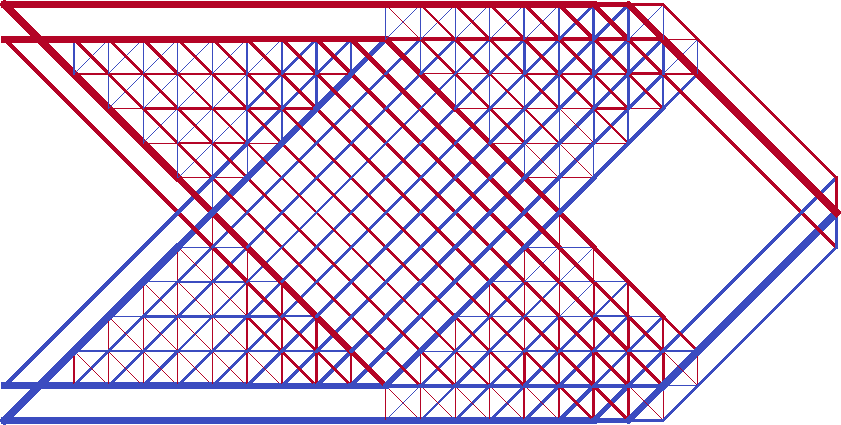
\includegraphics[width=\linewidth]{figures/06_DMO/00_cantilever_extremes/mono.pdf}
    \caption{$V=832.848$}
    \label{fig:06_cant_mono}
\end{marginfigure}


\begin{marginfigure}
    \centering
    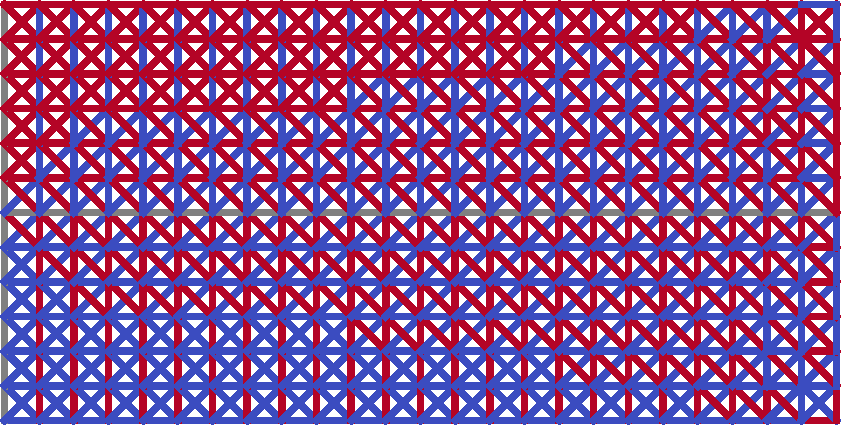
\includegraphics[width=\linewidth]{figures/06_DMO/00_cantilever_extremes/cell.pdf}
    \caption{$V=9832.935$}
    \label{fig:06_cant_BC_cell}
\end{marginfigure}

Now that we have set up the reference for better understand the optimization results, we perform the optimizations of the layout of the fixed topology module. Just for the first example we decided not to penalize intermediate weights, so $p=q=0$ and then $w=\alpha$. The optimized structure topology is shown in \figref{fig:06_fixed_module}a and \figref{fig:06_fixed_module}b, in wich we show also the weight distribution of the solution. Ath this stade, the optimized structure shows a volume $V = 1567.216$, a value that is not that far from the monolitic reference. however, this solution is non physical as many subdomains present intermediate dweights and we need to threshold the result. The thresolding value is set to 0.01, so any subdomains that have a weight w less than this value is considered empty. The result of the thresolding is presented in \figref{fig:06_fixed_module}d, in which we see that all weights are now set to 1. The resulting structure has a volume $V = 8808.671$, a very noticable increase due to the high number of intermediate weights shown by the solution of \figref{fig:06_fixed_module}b.

\todo{add frase on ramp curve}

\begin{figure*}
    \subcaptionbox{}{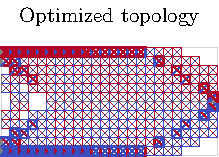
\includegraphics{figures/06_DMO/00_fixed_cells/top_00.pdf}}
    \hfill
    \subcaptionbox{$V = 1567.216$}{\includegraphics{figures/06_DMO/00_fixed_cells/weight_00.pdf}}
    \hfill
    \subcaptionbox{}{\includegraphics[height=3.5cm] {figures/06_DMO/00_fixed_cells/ramp_00.pdf}}
    \hfill
    \subcaptionbox{$V = 8808.671$}{\includegraphics{figures/06_DMO/00_fixed_cells/weight_00_PP.pdf}}
    \bigskip
    \subcaptionbox{}{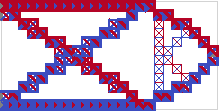
\includegraphics{figures/06_DMO/00_fixed_cells/top.pdf}}
    \hfill
    \subcaptionbox{$V = 1961.175$}{\includegraphics{figures/06_DMO/00_fixed_cells/weight.pdf}}
    \hfill
    \subcaptionbox{}{\includegraphics[height=3.5cm]{figures/06_DMO/00_fixed_cells/ramp.pdf}}
    \hfill
    \subcaptionbox{$V = 3414.214$}{\includegraphics{figures/06_DMO/00_fixed_cells/weight_PP.pdf}}
    \caption{}
    \label{fig:06_fixed_module}
\end{figure*}

To solve this problem, we set up a multi-phase RAMP interpolation where we simultaneously penalize mechanical properties (using the parameter $p$) and we artificailly icrease the volume (using the parameter $q$) of modules with intermediate weights. In this optimization we set $p=8$ and $q_\text{min}=-0.8$, and a continuation scheme is used on the $q$ parameter to gradually decresase it to the minimum value as already explained in \secref{sec:06_num_app}. The optimized structure topology with penaliized intermediate weights is shown in \figref{fig:06_fixed_module}e and \figref{fig:06_fixed_module}f and it has a volume $V = 1961.175$, a \qty{25}{\percent} volume increase with respect to the unpenalized structure. however we can clearly see how this solution present way less subdomains with intermediate weight and this is very reflected after the thresolding phase, in wich the volume is now $V=$, more thatn \qty{60}{\percent} less than the unpenalized structure. the difference between the structure of fig and fig could also be less , as in this case we see that the subdomains creates beams tat are made by only an elements and it is enough to transfer the loads. a finer subdivision of the initial structure could then beneficial.

Similarities with classic topology optimization. \sidecite{bendsoe_material_1999,sigmund_non-optimality_2016}

An additional test we performed was to . Int hese two test cases no perturbation is done on the initial starting point and alpha at iteration 0 is set to $\alpha = 0.5,\,\forall j,t $
\begin{figure}
    \subcaptionbox{}{\includegraphics[width=0.45\linewidth]{figures/06_DMO/00_fixed_cells_multiple/fig1-Topology_area.pdf}}
    \hfill
    \subcaptionbox{}{\includegraphics[width=0.45\linewidth]{figures/06_DMO/00_fixed_cells_multiple/fig1-Topology_topol.pdf}}
    \hfill
    \bigskip
    \subcaptionbox{}{\includegraphics[width=0.45\linewidth]{figures/06_DMO/00_fixed_cells_multiple/fig12-Module_withType_area.pdf}}
    \hfill
    \subcaptionbox{}{\includegraphics[width=0.45\linewidth]{figures/06_DMO/00_fixed_cells_multiple/fig12-Module_withType_topol.pdf}}
    \caption{}
    \label{fig:06}
\end{figure}
\subsection{Modules and layout optimization}
\begin{figure}
    \hspace*{\fill}
    \subcaptionbox{}{\includegraphics[width=0.45\linewidth]{figures/06_DMO/00_optimized_module/fig1-Topology.pdf}}
    \hfill
    \subcaptionbox{}{\includegraphics[width=0.3\linewidth]{figures/06_DMO/00_optimized_module/fig8-Module_Topology_001.pdf}}
    \hspace*{\fill}
    \caption{}
    \label{fig:06}
\end{figure}
\todo{tables with volume and phi and psi for different NT}

\begin{figure}
    \centering
    \includegraphics{figures/06_DMO/00_optimized_modules/kmeans.pdf}
    \caption{}
    \label{fig:06}
\end{figure}

\begin{figure*}
    \subcaptionbox{}{\includegraphics[width=0.3\linewidth]{figures/06_DMO/00_optimized_modules/nt2.pdf}}
    \hfill
    \subcaptionbox{}{\includegraphics[width=0.6\linewidth]{figures/06_DMO/00_optimized_modules/nt5.pdf}}
    \caption{}
    \label{fig:06}
\end{figure*}

\begin{marginfigure}
    \centering
    \includegraphics[width=\linewidth]{figures/06_DMO/00_optimized_modules/VL/nt=5VL.pdf}
    \caption{}
    \label{fig:06}
\end{marginfigure}

\subsection{A benchmark case study: a simply supported modular bridge}

\todo{difference with tugilimana, we take into account the buckling whensolving the first subproblem of module layout, we can have an empty subdomain andwe use a gradeint descent algo}

\begin{figure}
    \centering
    \includegraphics{figures/06_DMO/00_tug_bench/bench.pdf}
    \caption{}
    \label{fig:06}
\end{figure}

\begin{figure}
    \centering
    \includegraphics{figures/06_DMO/00_tug_bench_buck/buck.pdf}
    \caption{}
    \label{fig:06}
\end{figure}

\begin{figure*}
    \centering
    \includegraphics{figures/06_DMO/00_tug_bench_size/size.pdf}
    \caption{}
    \label{fig:06}
\end{figure*}
principalmente due motivi, cambia il metodo di rottura, non piu buckling e poi ho i vuoti

\subsection{Simply supported 3D beam}
\begin{margintable}
    \small
    \centering
    \begin{tabular}{cc}
    \toprule
    \textbf{Parameter}        & \textbf{Value} \\ \midrule
    $E$              & \qty{2.7}{GPa}     \\
    $\nu$            & 0.3   \\
    $\sigma_\text{c}, \sigma_\text{t}$ & $\pm $\qty{55}{MPa} \\
    $\rho$              & \qty{1.14}{\gram\per\cubic\centi\metre}   \\
    $P$              & \qty{100}{N}   \\
    \bottomrule
    \end{tabular}
    \caption{Material data used for the simply supported 3D beam optimization.}
    \label{tab:06_3D_supp_mat}
\end{margintable}

\begin{figure*}
    \hspace*{\fill}
    \subcaptionbox{}{\includegraphics[width=0.30\linewidth]{figures/06_DMO/00_print_topology/1_04_Topology_NLP_iso.png}}
    \hfill
    \subcaptionbox{}{\includegraphics[width=0.30\linewidth]{figures/06_DMO/00_print_topology/2_04_Topology_NLP_iso.png}}
    \hfill
    \subcaptionbox{}{\includegraphics[width=0.30\linewidth]{figures/06_DMO/00_print_topology/3_04_Topology_NLP_iso.png}}
    \hspace*{\fill}
    \bigskip
    \hspace*{\fill}
    \subcaptionbox{}{\includegraphics[width=0.30\linewidth]{figures/06_DMO/00_print_topology/1_04_Topology_NLP_XZ.png}}
    \hfill
    \subcaptionbox{}{\includegraphics[width=0.30\linewidth]{figures/06_DMO/00_print_topology/2_04_Topology_NLP_XZ.png}}
    \hfill
    \subcaptionbox{}{\includegraphics[width=0.30\linewidth]{figures/06_DMO/00_print_topology/3_04_Topology_NLP_XZ.png}}
    \hspace*{\fill}
    \caption{}
    \label{fig:06}
\end{figure*}

\begin{table}
    \centering
    \small
    \begin{tabular}{lx{1.8cm}x{1.8cm}x{1.8cm}x{1.8cm}}
        \toprule
    $N_\text{T}$ & --     & 1     &  2    &  3  \\ \midrule
    $N_\text{sub}$           &    1  &   36   &   36   &   36     \\
    $N_\text{opt}\;(N_\text{el})$  &  20 (1984) &  360 (12636)   &  204 (12636)   &  104 (12636)        \\
    $V$ [\unit{cm^3}] & 9.907 &  27.958 &   15.548  & 10.178    \\
    $V$ [\unit{\percent}] & 1.761 & 4.970&2.764 & 1.809    \\
    $\bar{\rho}$ [\unit{kg/m^3}] & 80.31 &226.65 &126.05 &82.51 \\
    C [\unit{J}]      &  3.71  &  5.20   &  6.21  & 4.141  \\
    $a_\text{max}$ [\unit{mm^2}]      & 37.61& 9.40  & 12.81  &   15.81     \\
    $\varphi$   &\qty{100.00}{\percent}&\qty{21.11}{\percent}&\qty{39.21}{\percent}&\qty{80.77}{\percent}  \\
    $\psi$& 1.00   &  0.47 &  0.66   & 0.87        \\
    t        & \hms{0;0;4}  &  \hms{0;1;18} & \hms{0;0;42} & \hms{0;10;22}   \\ \bottomrule
    \end{tabular}
    \caption{}
    \label{tab:06}
    \end{table}

\section{Conclusion}

% \setchapterpreamble[u]{\margintoc}
\glsresetall % reset glossary

\chapter{Design of real-size aeronautical wing structures} \label{chap:07}
\todo{tables always small}
Introduction

Ultralight trusses are a good design candidate for the design of innovative aerostructures thanks to their superior aeroelastic properties and stiffness-to-weight ratio \sidecite{cramer_elastic_2019}. These structures represent a natural application case for the discussed optimization formulations. \sidecite{opgenoord_aeroelastic_2018, opgenoord_design_2019} proposed a two-step sequential optimization algorithm to reduce the weight of a truss wing. Firstly, a ground structure with different nodal densities based on the stress field of the structure is generated and secondly, the cross-sectional areas are found using a sizing optimization algorithm that takes into account stress, local buckling, and aeroelastic constraints. \sidecite{shahabsafa_novel_2018} decided, instead, to tackle all the difficulties of the problem using a set of discrete cross-sectional areas and a sizing \gls{milo} algorithm. The algorithm is validated on a 315-bars wingbox ground structure, based on the \gls{crm}. In these studies, the adoption of a sizing optimization algorithm simplifies the numerical complexities associated with the problem. However, by solely focusing on modifying the component sizes, the opportunity to optimize the overall truss topology is missed, limiting the potential for further weight savings.

\section{3D CRM wingbox with multiple load cases}
In this section, the proposed strategy is used to optimize a real-size wingbox, to validate its ability to work on large, three-dimensional structures with more candidate members compared to the precedent test cases. The structure is based on the jig (undeformed) shape of the wingbox of the NASA \gls{crm} \sidecite{brooks_benchmark_2018}. The structure is submitted to three different load cases: +2.5 g maneuver (LC\_1), -1 g maneuver (LC\_2), and cruise with gust +1.3 g (LC\_3). The nodes of the bounding volume and the loads used are provided by \sidecite{fakhimi_discrete_2021}, where a detailed discussion on how they are evaluated can be found. The ground structure of the test case is presented in \figref{fig:07_crm315_x0}.

The material used for the optimization is an aluminum alloy with Young's modulus of \qty{69}{\GPa}, density of \qty{2.7}{\gram/\cm^3}, and yield stress equal to $\pm$\qty{270}{\MPa} (see \tabref{tab:07_CRM_mat}). To ensure a conservative design, we incorporated safety factors (\textit{sf}) associated with each load case. These safety factors were integrated into the formulation by reducing the maximum stress and buckling allowables by factors of 1.5, 1.5, and 2.67 for the three considered load cases, respectively. No bounds constraints are imposed on the nodal displacements of the structure and the cross-sections are assumed circular with the cross-sectional buckling parameter $s = \pi E/4$. The optimization is carried only on the wingbox, the internal structure of the wing, and there is no influence of the skin on the optimization.
\begin{margintable}
    \small
    \centering
    \begin{tabular}{cc}
    \toprule
    \textbf{Parameter}        & \textbf{Value} \\ \midrule
    $E$              & \qty{69}{GPa}     \\
    $\sigma_\text{c}, \sigma_\text{t}$ & $\pm $\qty{270}{MPa} \\
    $\rho$              & \qty{2.7}{\gram\per\cubic\centi\metre}   \\
    \bottomrule
    \end{tabular}
    \caption{Material data used for the CRM optimization.}
    \label{tab:07_CRM_mat}
\end{margintable}

\subsection{Advanced thresholding}
As the \gls{crm} is a large and thin structure that presents a noticeable difference in load magnitude between the tip and the root of the wingbox, the quantities of interest of the optimization span different orders of magnitude (from \unit{m^2} to \unit{mm^2}, and\marginnote{\eqref{eq:04_thr} reads: $$a_i<a_{\text{thr}} \; \forall i, \text{ with }a_{\text{thr}} = \chi \; \max(\tilde{\vect{a}}^*)$$} from \unit{MN} to \unit{N}). For that reason, the choice of the cross-sectional area threshold value $\chi$ defined in \eqref{eq:04_thr} and used to simplify the initial \gls{nlp} ground structure is crucial. Taking a high value (such as $\chi = 10^{-4}$, restraining the solution from \unit{m^2} to \unit{cm^2}) would mean possibly canceling out bars fundamental for the nodal force equilibrium in the less loaded part of the wing (wing tip and the central part of the wing's sections near the root). By contrast, a low value (such as $\chi=10^{-9}$) would permit the correct simulation of the mechanical response of the structure, but it would lead to a very high number of candidate bars and, thus, longer optimizations and convergence difficulty for the \gls{nlp} phase. For that reason, $\chi$ is set to an average value ($\chi=10^{-6}$), eliminating all the bars under the value $a_{\text{thr}}=\chi \; \max(\vect{a})$, but an additional check is performed before proceeding to the thresholding. The bars under the threshold $a_{\text{thr}}$ are sorted in ascending order of cross-sectional area and, starting from the smallest one, we iteratively check via a \gls{fea} that the difference between the force and displacement fields before and after the bar removal is below than a certain bound. In the present study we used the following: $\norm{\Delta q}_{\infty}<\qty{10}{N}$ and $\norm{\Delta U}_{\infty}<\qty{1}{cm}$.


\subsection{Numerical application}

\begin{table}
    \small
    \centering
    \begin{tabular}{ccc}
    \toprule
    \textbf{Quantity} & \textbf{CRM-315} & \textbf{CRM-2370} \\ \midrule
    N$_{\text{el}}$          & 315               & 2370               \\
    N$_{\text{opt}}$           & 257                  &  1127              \\
    V [\unit{\meter^3}]             &  7.90                 &  7.44             \\
    V [\unit{\%}]             &   \qty{1.309}{\%}                & \qty{1.232}{\%}               \\
    Mass [\unit{\tonne}]               &   21.342                & 20.092     \\
    a$_{\text{max}}$ [\unit{\meter^2}]           &  0.198                 & 0.208              \\
    C$_\text{LC\_1}$ [\unit{\mega \joule}]                &  3.23                 &  3.17              \\
    C$_\text{LC\_2}$ [\unit{\mega \joule}]                &   1.28                &  1.27              \\
    C$_\text{LC\_3}$ [\unit{\mega \joule}]                &   0.76                &  0.74              \\
    t [\unit{\second}]                & 147                  & 3189   \\ \bottomrule            
    \end{tabular}
    \caption{Numerical results of the optimization of the CRM with two different ground structures.}
    \label{tab:wing-res}
    \end{table}
    
    \begin{figure*}
        \centering
        \subcaptionbox{\label{fig:07_crm315_x0}}{\includegraphics[width=0.45\linewidth]{figures/07_aeronautic/14a_00_Topology_x0_iso.png}}
        \bigskip
        \subcaptionbox{\label{fig:07_crm2317_x0}}{\includegraphics[width=0.45\linewidth]{figures/07_aeronautic/14b_00_Topology_x0_iso 2370.png}}
        \caption{(a) Ground structure of the CRM-315 test case; (b) Ground structure of the CRM-2370 test case. The cross-sectional areas shown in the two sub-figures represent the starting point of the optimizations.}
        \label{fig:07_crm}
    \end{figure*}
    
    \begin{figure}
        \centering
        \includegraphics[width=0.8\linewidth]{figures/07_aeronautic/15_04_Topology_NLP_iso.png}
         \caption{Optimized topology of the CRM-315 with 257 active bars.}
        \label{fig:07_crm315}
    \end{figure}
    
    Two different discretizations are considered for the optimization. The proposed algorithm is firstly tested on the same ground structure provided by Fakhimi \etal \sidecite{fakhimi_discrete_2021}, composed of $N_{\text{el}}=315$ candidate members (CRM-315). The second discretization is obtained by refining the 315-bar ground structure, evaluating the midpoints of every member, and connecting them with first-order connectivity. We obtain $N_{\text{el}}=2370$ candidate members (CRM-2370). The loads and the boundary conditions are applied on the same nodes of the ground structure for the two studied ground structures. The cross-sectional areas of the starting point of the CRM-315 and the CRM-2370 are set to \qty{0.0001}{m^2} and they are shown in \figref{fig:07_crm}. Only one single start point is used for these two examples as the proposed two-step strategy with reinitialization already proved in the previous sections to reduce the starting point influence on the optimization result. The resolution algorithm used is 2S-5R. The numerical results of the optimization for the two different discretizations are reported in \tabref{tab:wing-res}. 
    
    The optimized CRM-315 structure shows a mass of \qty{21.342}{\tonne}, a \qty{27.01}{\%} reduction compared to the solution with discrete cross-section areas found by Fakhimi \etal \sidecite{fakhimi_discrete_2021} (\qty{29.238}{\tonne}). Other than the substantial difference in the modelization of the cross-section areas, the mass reduction could be explained by the fact that the proposed algorithm has a zero lower bound on cross-sectional areas, thus permitting the topology of the structure to change: the 2S-5R solution shows 257 active bars out of 315 at convergence (see \figref{fig:07_crm315}). In contrast, the \gls{milo} problem solved by Fakhimi \etal \cite{fakhimi_discrete_2021} is employed as a sizing optimization algorithm with fixed topology (and thus 315 active members in the optimized design). A more detailed comparison could not be performed as the authors did not share the values of the cross-sectional areas of their solution. 
    
    The volume fraction of the solution is \qty{1.313}{\percent} and the minimum slenderness ratio $\lambda$ (ratio between the length and the radius of gyration of the bar) of a bar is 14.96, which is compatible with the truss modelization used to discretize the wingbox volume. The execution time of the optimization is \qty{19}{s} for the \gls{slp} step and \qty{128}{s} for the \gls{nlp} step, for a total of \qty{147}{s} on a regular notebook, compared to the over four days of optimization of Fakhimi \cite{fakhimi_discrete_2021} on a desktop workstation. The iteration history curves of the optimization are plot in \figref{fig:07_c2}.

    \begin{figure*}
        \centering
        \subcaptionbox{}{\includegraphics[width=0.49\linewidth]{figures/07_aeronautic/19a_v_hist_315.pdf}}
        \bigskip
        \subcaptionbox{}{\includegraphics[width=0.49\linewidth]{figures/07_aeronautic/19b_c_hist_315.pdf}}
        \caption{Iteration history of the CRM-315 example solved with the 2S-5R algorithm. (a) objective function history for the SLP and NLP step. The sharp increases in the objective function during the SLP step correspond to the reinitialization calls. (b) constraint violation for the NLP step.}
        \label{fig:07_c2}
    \end{figure*}

\paragraph{Maximum displacements constraints}

agiamo sulla stiffness, gaurda i valori di compliance come scendono

\begin{table}
    \small
    \centering
    \begin{tabular}{ccccc}
    \toprule
    $\bm{Z}_\ell\:[\text{m}]$ & 1&2&3&--\\ \midrule
    V [\unit{\meter^3}]&  26.70&13.78&9.39&7.90\\
    V [\unit{\%}]&   \qty{4.421}{\%}   & \qty{2.283}{\%}&\qty{1.556}{\%}&\qty{1.309}{\%}  \\
    Mass [\unit{\tonne}]  &72.086&37.218&25.363&21.342\\
    a$_{\text{max}}$ [\unit{\meter^2}]&  0.615    & 0.293&0.197&0.198\\
    C$_\text{LC\_1}$ [\unit{\mega \joule}]   &  1.05    &  1.96&2.79& 3.23\\
    C$_\text{LC\_2}$ [\unit{\mega \joule}]   &   0.37   &  0.71&1.04& 1.28\\
    C$_\text{LC\_3}$ [\unit{\mega \joule}]   &   0.26   &  0.47&0.67& 0.76\\

    \bottomrule
    \end{tabular}
    \caption{remember \todo{put here the span of the wing}}
    \label{tab:07_disp}
\end{table}

\begin{figure*}
    \centering
    \includegraphics[width=\linewidth]{figures/07_aeronautic/00_dispalcements/disp.pdf}
     \caption{}
    \label{fig:07_disp_sol}
\end{figure*}

\paragraph{Multiple materials}
\todo{complete with Ashby charts on cost and co2 evaluation}

\begin{table}
    \small
    \centering
    \begin{tabular}{ccccc}
    \toprule
    \textbf{Material} &\textbf{Aluminium}&\textbf{Titanium}&\textbf{Steel}&\textbf{Pultruted CFRP}\\ \midrule
    $E$& \qty{69}{GPa}&\qty{120}{GPa}&\qty{210}{GPa}&\qty{150}{GPa}     \\
    $\sigma_\text{c}, \sigma_\text{t}$ & $\pm $\qty{270}{MPa}&$\pm $\qty{880}{MPa}&$\pm $\qty{355}{MPa}&+1200,\qty{-880}{MPa} \\
    $\rho$& \qty{2.7}{\gram\per\cubic\centi\metre}&\qty{4.5}{\gram\per\cubic\centi\metre}&\qty{7.8}{\gram\per\cubic\centi\metre}&\qty{1.6}{\gram\per\cubic\centi\metre}   \\
    \unit{kg CO^2_e\per\kilo\gram}&12.5&47.0&5.0&34.5 \\
    \unit{\$\per\kilo\gram}&2.2&23.5&6.3&40.5\\
    \bottomrule
    \end{tabular}
    \caption{remember \todo{put here the span of the wing}}
    \label{tab:07_materials_data}
\end{table}

\sidecite{ashby_materials_1999}

\gls{cfrp}

\begin{table}
    \small
    \centering
    \begin{tabular}{ccccc}
    \toprule
    \textbf{Material} &\textbf{Aluminium}&\textbf{Titanium}&\textbf{Steel}&\textbf{Pultruted CFRP}\\ \midrule
    V [\unit{\meter^3}]&7.90&4.53&10.97&3.67\\
    V [\unit{\%}]&\qty{1.309}{\%}&\qty{0.749}{\%}&\qty{1.816}{\%}&\qty{0.607}{\%}\\
    Mass [\unit{\tonne}]& 21.342&20.372&86.112&5.868\\
    a$_{\text{max}}$ [\unit{\meter^2}]&0.198&0.088&0.154&0.86\\
    C$_\text{LC\_1}$ [\unit{\mega \joule}]&3.23&4.88&1.19&4.39\\
    C$_\text{LC\_2}$ [\unit{\mega \joule}]&1.28&1.94&0.47&1.73\\
    C$_\text{LC\_3}$ [\unit{\mega \joule}]&0.76&1.15&0.28&1.03\\
    $Z_\ell\:[\text{m}]$&4.10&5.97&1.42&5.31\\
    Cost [\unit{\tonne CO^2_e}]&266.7&957.5&430.6&202.4\\
    Cost [\unit{k\$}]&46.9&478.7&542.5&237.6\\
    \bottomrule
    \end{tabular}
    \caption{remember \todo{put here the span of the wing}}
    \label{tab:07_materials}
\end{table}

ovviamente qui si tiene in conto solo il materiale, ma il peso inferiore su un aero permette di risparmiare veramente molto di piu

\begin{figure*}
    \centering
    \includegraphics[width=\linewidth]{figures/07_aeronautic/00_materials/mat.pdf}
     \caption{}
    \label{fig:07_mat_sol}
\end{figure*}

\todo{grafico co2 soldi per materiale}

\begin{marginfigure}
    \centering
    \includegraphics[width=\linewidth]{figures/07_aeronautic/00_co2eq/co2_dollar.pdf}
    \caption{}
    \label{fig:07}
\end{marginfigure}

\todo{grafico volume/resistenza specifica}

\paragraph{Enriching the mesh}
\begin{figure*}
    \centering
    \includegraphics[width=\linewidth]{figures/07_aeronautic/16_wing_opt/wing_opt.pdf}
     \caption{Maximum stress constraint value (left) and buckling constraint value (right) plotted on the deformed shape of the optimized design (undeformed shape in light grey) of CRM-2370 for the three load cases: +2.5 g maneuver (a), -1 g maneuver (b), and cruise with gust (+1.3 g) (c). The maximum $z$ tip deflection is \qty{4.167}{m}, \qty{-2.953}{m}, and \qty{1.948}{m}, respectively.}
    \label{fig:07_wing_opt}
\end{figure*}
The mass of the optimized CRM-2370 structure is \qty{20.092}{\tonne}, a \qty{1.318}{\tonne} reduction compared to the CRM-315 (\qty{-6.2}{\%}). Additionally, if we compare the compliance of the three load cases (see \tabref{tab:wing-res}), we notice how the solution of CRM-2370 is not only lighter but also stiffer, suggesting in general a more efficient structure topology. The maximum \todo[sostituiscci con Zell] z tip deflection of the wingbox is \qty{4.167}{m}, \qty{-2.953}{m}, \qty{1.948}{m} for the three considered load cases, respectively. There are 1127 active bars in the optimized design, and the whole optimization took \qty{3189}{s} (\qty{1911}{s} for the \gls{slp} step, \qty{1278}{s} for the \gls{nlp} step). The iteration history curves of the optimization are plot in \figref{fig:07_c3}. In \figref{fig:07_wing_opt} the normalized maximum stress and buckling constraints are plotted on the deformed shape of the three load cases. We notice how in general the topology of the two external "spars" is shaped after the +2.5 g load case, while the interior of the wingbox is made by a thinner truss constrained by buckling. 

\begin{figure*}
    \centering
    \subcaptionbox{}{\includegraphics[width=0.49\linewidth]{figures/07_aeronautic/20a_v_hist_2370.pdf}}
    \bigskip
    \subcaptionbox{}{\includegraphics[width=0.49\linewidth]{figures/07_aeronautic/20b_c_hist_2370.pdf}}
    \caption{Iteration history of the CRM-2370 example solved with the 2S-5R algorithm. (a) objective function history for the SLP and NLP step. The sharp increases in the objective function during the SLP step correspond to the reinitialization calls. (b) constraint violation for the NLP step.}
    \label{fig:07_c3}
\end{figure*}

\paragraph{Active mechanical constraints}
To better understand which mechanical phenomena is the most constraining for the bars of the solution, we present in \figref{fig:fail-crm} a graph where the normalized stress criterion $\vect{c_s}=\max{\left(-\vect{q} \; \textit{\textbf{sf}}/\sigma_c \vect{a},\vect{q} \; \textit{\textbf{sf}}/\sigma_t \vect{a}\right)}$ and the normalized buckling criterion $\vect{c_b}=\vect{q}\; \textit{\textbf{sf}}/\vect{q}_{\text{crit}}$ are plotted against each other. Every point in the scatter plot represents the members of the solution of the \gls{slp} and the \gls{nlp} steps that show at least a charge of 1N (931 out of 1127 members). This threshold is applied as at the end of the NLP step some members present a very small section, creating numerical problems when evaluating the stress and buckling criteria. All the \gls{slp} members activate either the maximum stress or buckling limit, while 68 out of 931 \gls{nlp} members are located in the center of the graph ($c_s<0.95$ and $c_b<0.95$). We speculate that this behavior is due to the inclusion of the kinematic compatibility constraint in the \gls{nlp} algorithm: the cross-sectional area of these bars is chosen to comply with the global displacements. In \tabref{tab:07_constrNLP}, a summary of the active mechanical failure constraints (buckling, tensile stress, and compressive stress) present in the NLP solution. The table showcases the number of active constraints categorized by constraint type and load case. The optimized design encompasses a total of 930 active mechanical failure constraints for 863 bars (931 minus the 68 bars constrained by kinematic compatibility). This suggests that certain members are concurrently subject to multiple failure constraints across different load cases. An additional observation is that the design of the solution is primarily influenced by local buckling and compressive failures, especially under the +2.5 g load case (LC\_1).

\begin{figure}
    \centering
    \includegraphics[width=0.8\linewidth]{figures/07_aeronautic/18_failure new/failure_max.pdf}
     \caption{Normalized buckling and maximum stress constraint values for the optimized CRM-2370 structure after the SLP and the NLP optimization steps.}
    \label{fig:fail-crm}
\end{figure}

\begin{table}
\small
\centering
\begin{tabular}{lS[table-format=3.0]S[table-format=3.0]S[table-format=3.0]S[table-format=3.0]S[table-format=3.0]}
\toprule
                     & \textbf{LC\_1} & \textbf{LC\_2} & \textbf{LC\_3} & \textbf{Tot.} \\ \midrule
\textbf{Buckling}    & 281           & 145           & 143           & 569           \\
\textbf{Tension}     & 56            & 3             & 4             & 63            \\
\textbf{Compression} & 286           & 6             & 6             & 298           \\
\midrule
\textbf{Tot.}        & 623           & 154           & 153           & 930          \\
\bottomrule
\end{tabular}
\caption{Number of active mechanical failure constraints for the CRM-2370 optimized design per type of constraint (rows) and per load case (columns).}
\label{tab:07_constrNLP}
\end{table}

\section{NACA 0012 drone wing}

\subsection{Numerical implementation}

\subsection{Meshing irregular volumes}
\begin{figure*}
    \centering
    \includegraphics[width=\linewidth]{figures/07_aeronautic/00_naca_howtomesh/MESH.pdf}
     \caption{}
    \label{fig:07_howto}
\end{figure*}

\subsection{Definition of the repetitive zones}

\subsection{Numerical application}

\begin{table}
    \centering
    \small
    \begin{tabular}{lx{1.8cm}x{1.8cm}x{1.8cm}x{1.8cm}}
        \toprule
    $N_\text{T}$ & --     & 1     &  2    &  3  \\ \midrule
    $N_\text{sub}$           &    1  &   36   &   36   &   36     \\
    $N_\text{opt}\;(N_\text{el})$  &  20 (1984) &  360 (12636)   &  204 (12636)   &  104 (12636)        \\
    $V$ [\unit{cm^3}] & 9.907 &  27.958 &   15.548  & 10.178    \\
    $V$ [\unit{\percent}] & 1.761 & 4.970&2.764 & 1.809    \\
    $\bar{\rho}$ [\unit{kg/m^3}] & 80.31 &226.65 &126.05 &82.51 \\
    C [\unit{J}]      &  3.71  &  5.20   &  6.21  & 4.141  \\
    $a_\text{max}$ [\unit{mm^2}]      & 37.61& 9.40  & 12.81  &   15.81     \\
    $\varphi$   &\qty{100.00}{\percent}&\qty{21.11}{\percent}&\qty{39.21}{\percent}&\qty{80.77}{\percent}  \\
    $\psi$& 1.00   &  0.47 &  0.66   & 0.87        \\
    t        & \hms{0;0;4}  &  \hms{0;1;18} & \hms{0;0;42} & \hms{0;10;22}   \\ \bottomrule
    \end{tabular}
    \caption{Numeric results of the parametric study on the influence of the number of modules $N_\text{T}$ on the NACA 0012 drone wing.}
    \label{tab:07}
    \end{table}

\section{Conclusion}

% \include{chapters/8_3D_printing}

% \include{chapters/9_conclusion}

%----------------------------------------------------------------------------------------

% \backmatter % Denotes the end of the main document content
% \setchapterstyle{plain} % Output plain chapters from this point onwards

%----------------------------------------------------------------------------------------
%	BIBLIOGRAPHY
%----------------------------------------------------------------------------------------

% The bibliography needs to be compiled with biber using your LaTeX editor, or on the command line with 'biber main' from the template directory

\pagelayout{margin} % Restore margins
\printbibliography[heading=bibintoc, title=Bibliography] % Add the bibliography heading to the ToC, set the title of the bibliography and output the bibliography note
\pagelayout{wide} % No margins


%----------------------------------------------------------------------------------------
%	INDEX
%----------------------------------------------------------------------------------------

% The index needs to be compiled on the command line with 'makeindex main' from the template directory

\printindex % Output the index


% \appendix % From here onwards, chapters are numbered with letters, as is the appendix convention

% \pagelayout{wide} % No margins
% \addpart{Appendix}
% \pagelayout{margin} % Restore margins

% \chapter{Geometry generation for ultra-light structures}


\end{document}